\title{Master of Science \\ Organizational Management (Human Services) \\ Graduate Portfolio}
\author{Dustin Kindred \\ Chadron State College}
\date{\today}

\documentclass[12pt,titlepage]{article}
\usepackage[final]{pdfpages}
\usepackage[letterpaper, margin=1in]{geometry}
\usepackage[hidelinks]{hyperref}
% todo: Make Active navigation Links in Table of Contents
\renewcommand*\contentsname{Table of Contents}
\begin{document}
\maketitle
\tableofcontents
\newpage
\section{Part I}

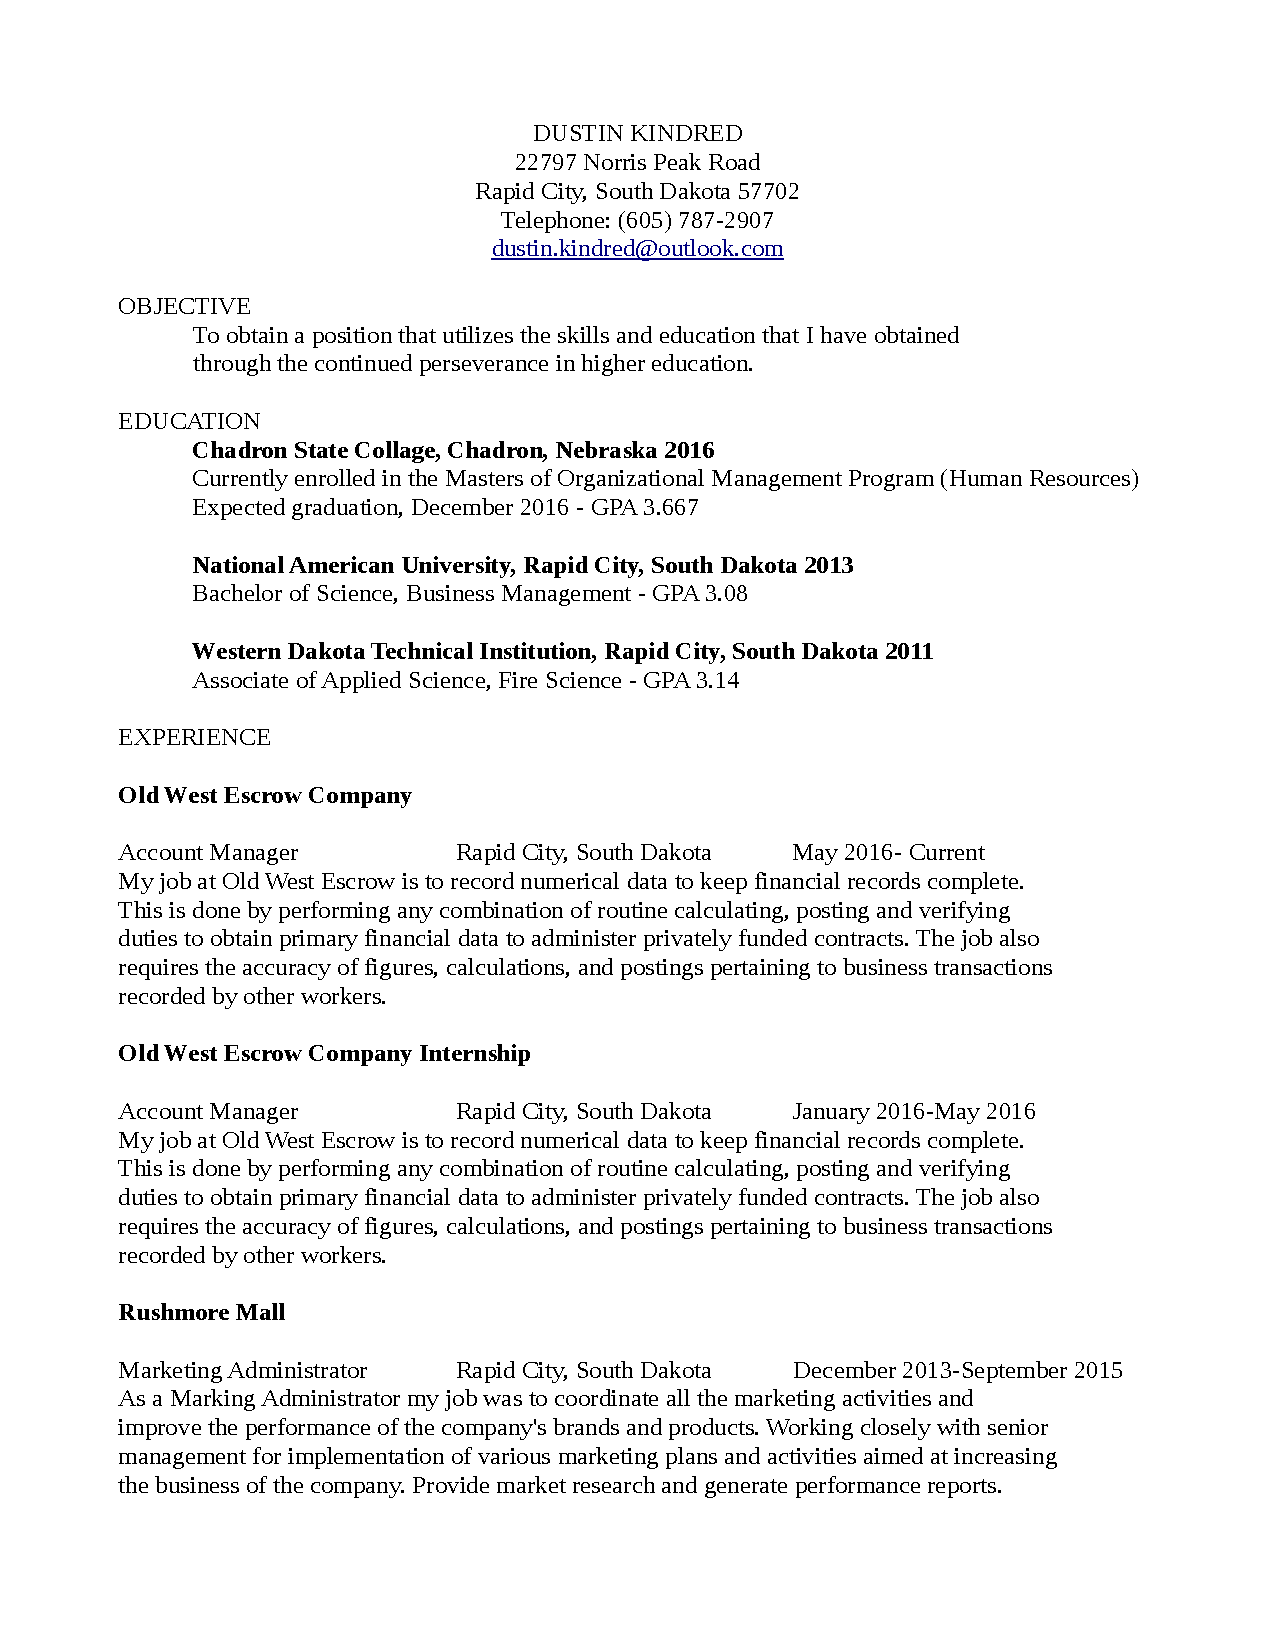
\includepdf[pages=1,pagecommand={\subsection{Resume}}]{resume.pdf}
\includepdf[pages=2-]{resume.pdf}
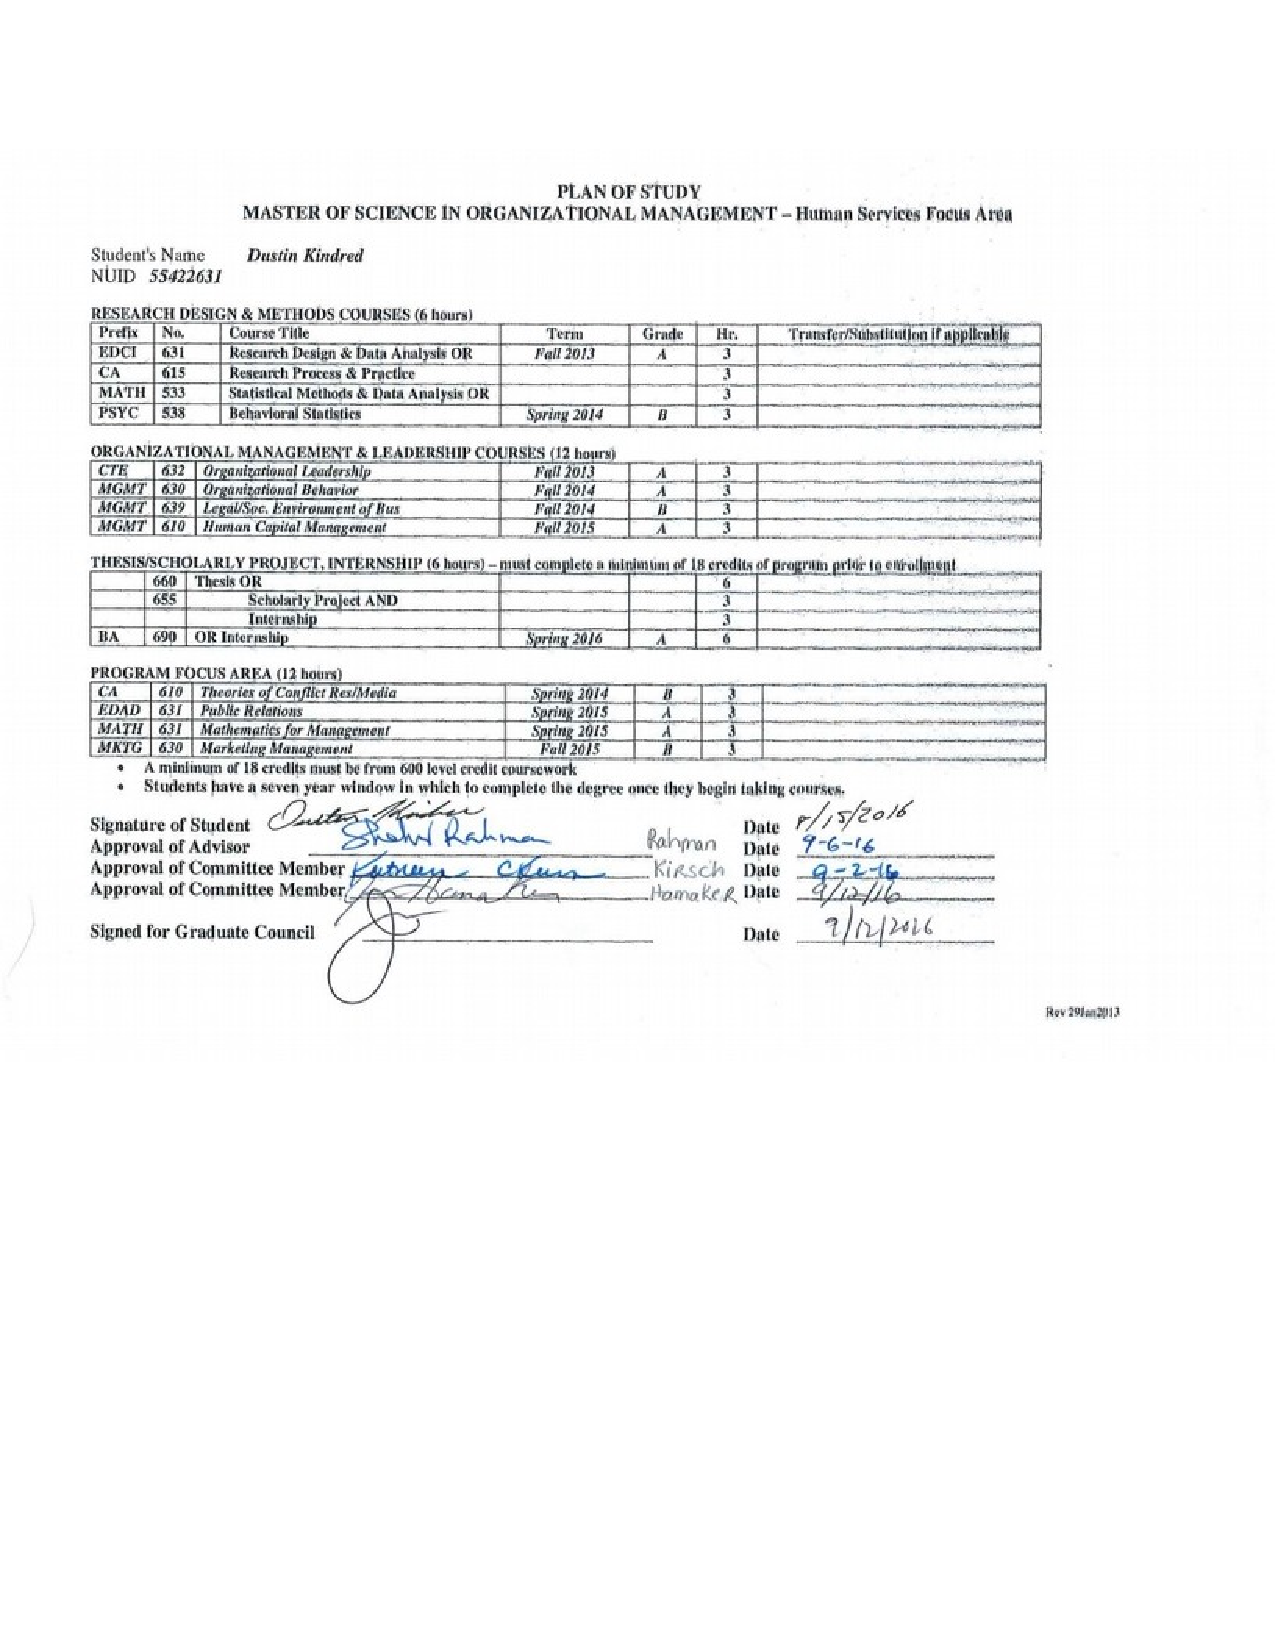
\includepdf[pages=1,pagecommand={\subsection{Plan of Study}}]{planofstudy.pdf}

% Part 2
\section{Part II}
% Part 2 Research Design
\subsection{Research Design and Data Analysis}
\subsubsection{Reflections}
\paragraph {}
Research and design analysis was an interesting class. The class was also my most feared class that could have taken. I am not a prolific writer by any means. My writing currently lacks style and the flare that I have come to expect when reading academic papers. However, this class helped a great deal in regards to feeling comfortable with my writing style. The areas in writing that I lacked then are still my faults on my writing today I am just getting better at spotting the errors. This was not the only purpose of the class. The purpose was to understand the basic research and design process to better understand the methodologies used in academic research. The course met this purpose and exceeded expectations. Dr. Blundell was excellent with the delivery of her instruction and returned assignments with helpful notes to the student showing where we could perform better and expand on our ideas.
\paragraph {}
The current course objectives were to comprehend research design and statistical analysis while applying common descriptive comparative and predictive procedures to selected data. The last objective was to create an original research problem and develop an integrated literature review and propose related research from this plan. All objectives I felt were met throughout the course. The course was a nice break-in course for advanced behavioral statistics giving a nice introduction to the class that was taken at a later time. Because we went through the fundamentals of statistical data and what it means as we read other academic reports I was able to infer whether I needed more material to back my claims as we went through an original research problem.
\paragraph {}
For the original problem I chose to focus in an area that I was currently working. I was working in emergency mental health confronted with an organizational goal of reducing arrests among the mentally ill community. Here I struggled a bit at refining my research problem into quantifiable terms. At first the problem was too vague and gave little to a researchable answer. Dr. Blundell was excellent at providing direction in this regard. After refinement I choose to narrow the topic to the use of intervention teams in conjunction with psychiatric emergency services. After performing the literature review process and writing the final paper I was confident to say that the issue still needs more research to solve the specific topic. While working in the capacity of my position I would have loved to be able to actually perform the specific study and feel that this class enable me to exude the confidence needed to go forward with the study if I had the chance.% Fall 2013
% Syllabus
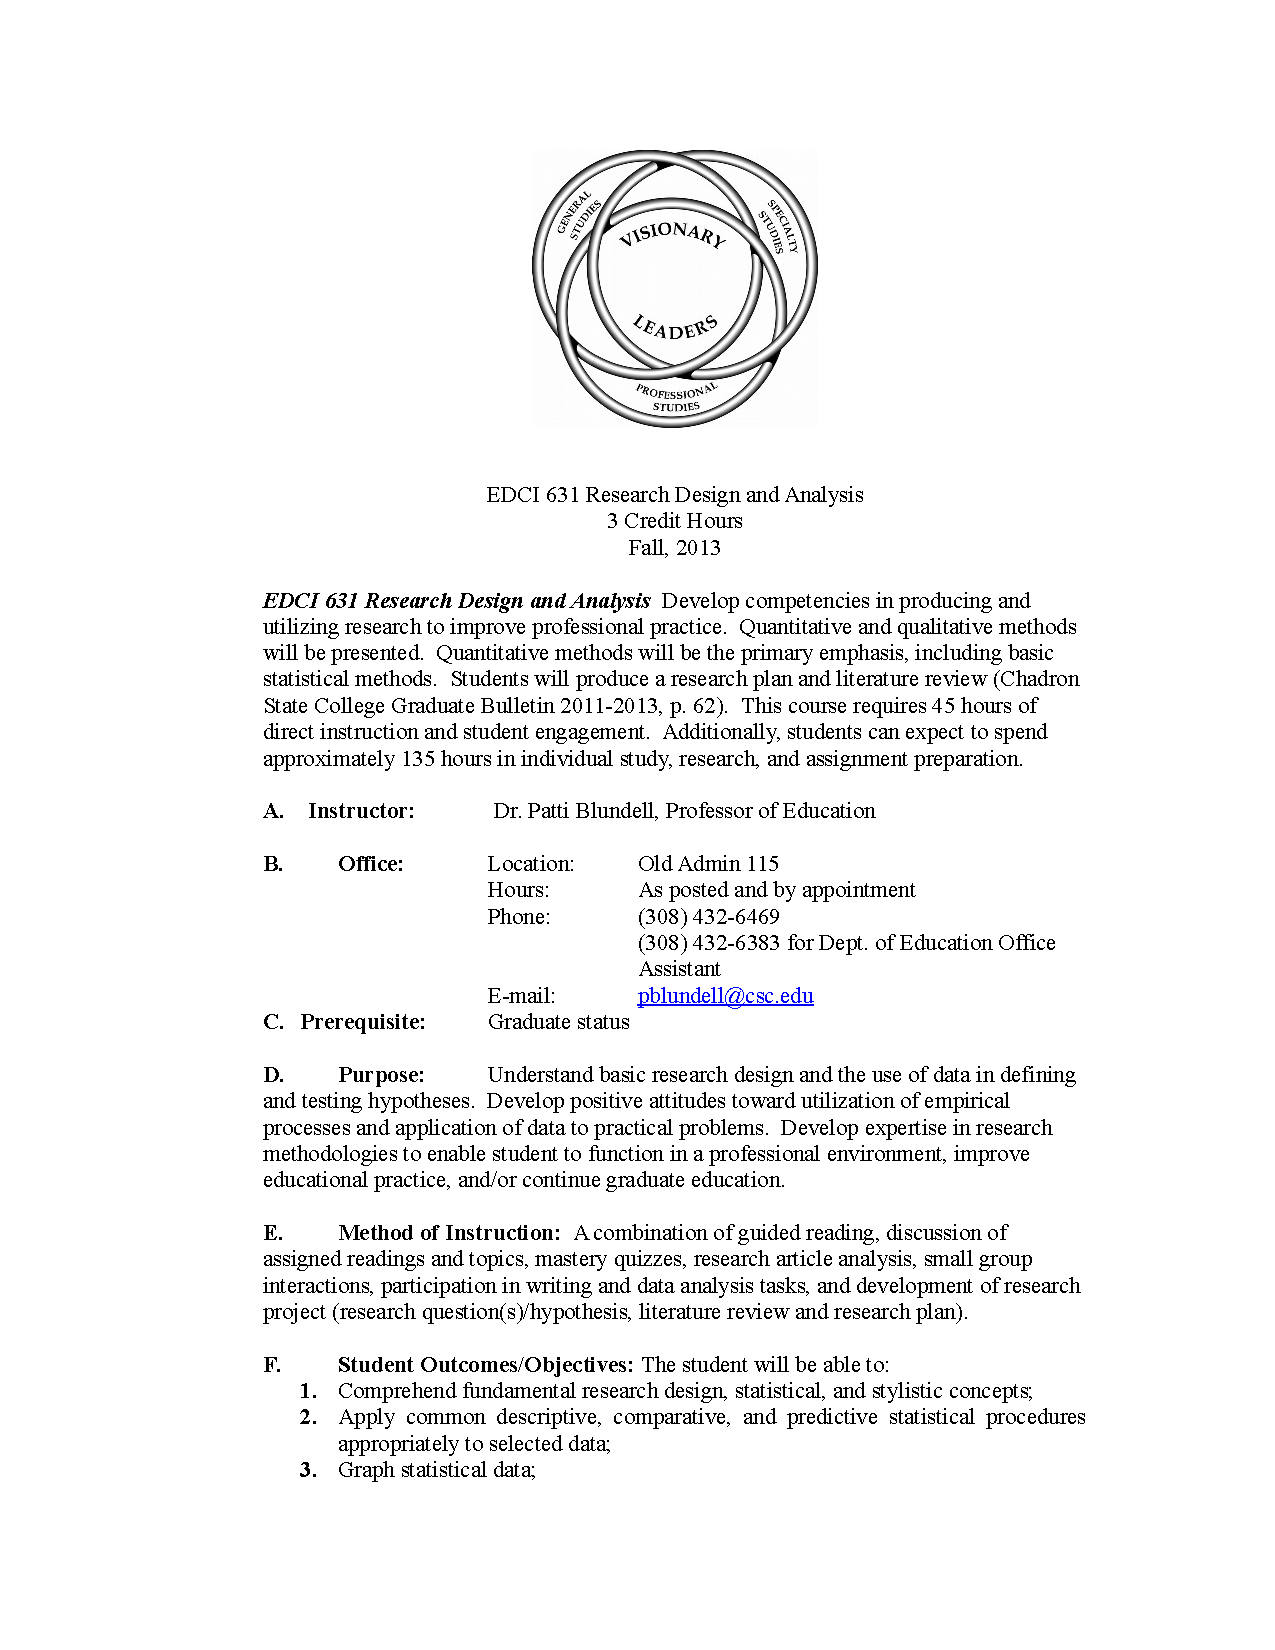
\includepdf[pages=1,pagecommand={\subsubsection{Research Design and Data Analysis Syllabus}}]{EDCI631syllabusfall13.pdf}
\includepdf[pages=2-]{EDCI631syllabusfall13.pdf}

% Work Examples
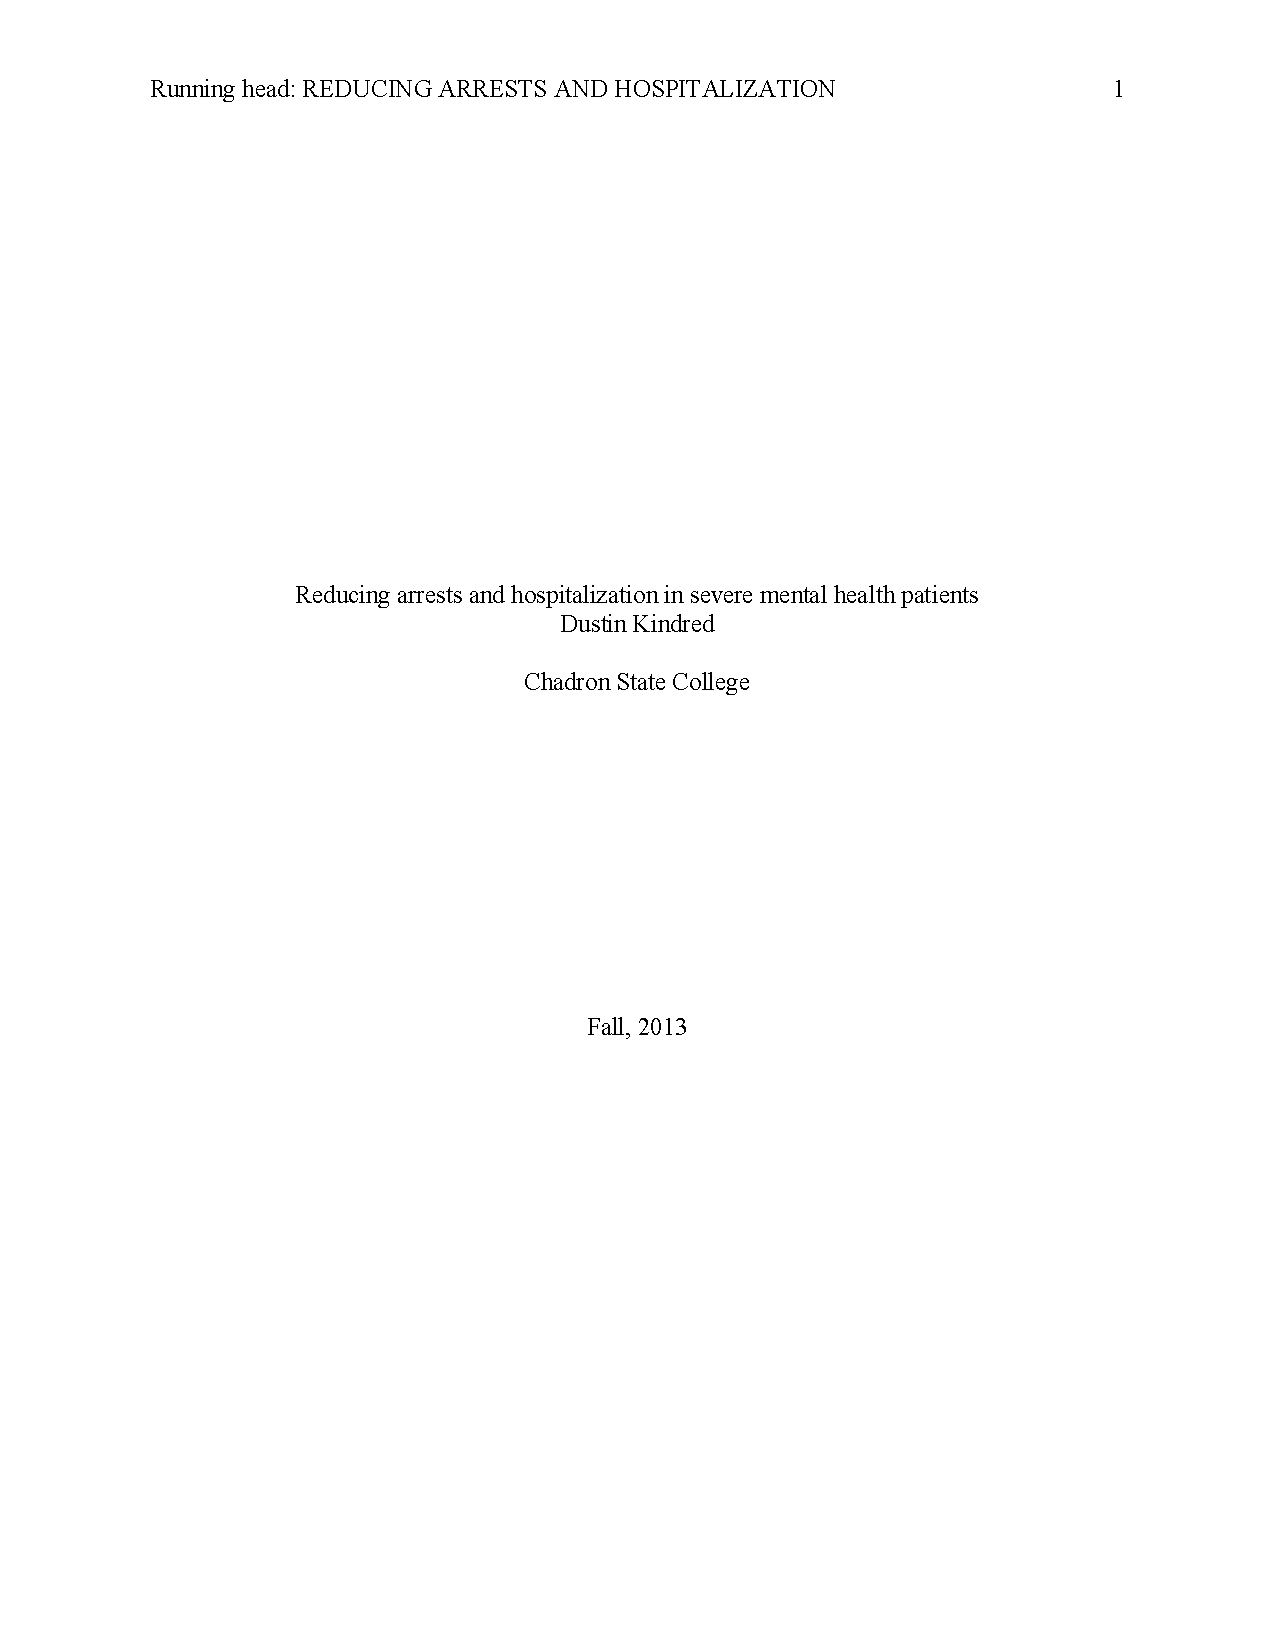
\includepdf[pages=1,pagecommand={\subsubsection{Work Examples}}]{Reducing_Arrests_&_Hospitalization_working_draft.pdf}
\includepdf[pages=2-]{Reducing_Arrests_&_Hospitalization_working_draft.pdf}

% Part 2 Org Leadership
\subsection{Organizational Leadership}
\subsubsection{Reflections}
% Start of Reflections
\paragraph {}
Organizational Leadership or CTE 632 was easily one of my favorite classes that I had taken and was looking forward to participating in. I felt that this class was one of the premier cornerstone classes to the degree program. I was happy that the class didn't have a required textbook rather we used a variety of different readings that Dr. Nealeigh had provided to us as we went through the different leadership styles. I found this teaching methodology more interesting and engaging than using a textbook. I also really like the book project where we had read a book on an inspirational leader and compare them to leadership styles found in other books. This helped the class feel engaging through applied critical thinking.
\paragraph {}
I learned that there are 6 leadership styles that are commonly practiced. Even though we have these six styles we may fall into the trap of conforming to just one style and make the best of it. However, this is not advantageous to us as leaders. As leaders we need to recognize the situation and then apply the correct style to the situation. A great example would assume that I fall into the democratic style of leadership. This is a great style and forces everyone to work and contribute together. This style ,however, is not beneficial in emergency situations. In these scenarios the leader needs to make quick direct decisions based on the rapidly evolving conditions. In this situation I would need to switch gears and become a coercive leader. As future leaders we cannot convince ourselves that there is only one style of leadership that is the best for everyone. We need to become fluid and adapt as needed.
\paragraph {}
During the course we also learned about organizations and how they are setup with a vertical leadership structure for horizontal structure. Organizations can also be compartmentalized or non-compartmentalized. Again, these hierarchies are based on what works for the organization and does not work for every situation. I have found that in smaller organizations it will make more sense to deploy the horizontal or flat structures.
\paragraph {}
Perhaps the best part of the class was reinforcing the concepts of power and empowerment as it relates to employees and how employees react to these methods. I particularly take to the concepts of employee empowerment as it relates to job function. As leaders we need to recognize employees that are able to expand beyond their designed job functions to encourage growth and job satisfaction. We also need to understand that job enlargement can also add undue stress in the workplace when we enlarge too much. In situations such as this we need to consider if the employee needs to take on a new job title to recognize the work they are doing for the organization or if we need to hire other employees to reduce the workload balance conundrum. In either situation this class has giving tools that will be used everyday. The theories and concepts may not always be on the forefront of the mind daily, but are well instilled in my leadership style. Currently my leadership style is a mixture of authoritative and democratic. % Start Syllabus
\newgeometry{top=.3in}
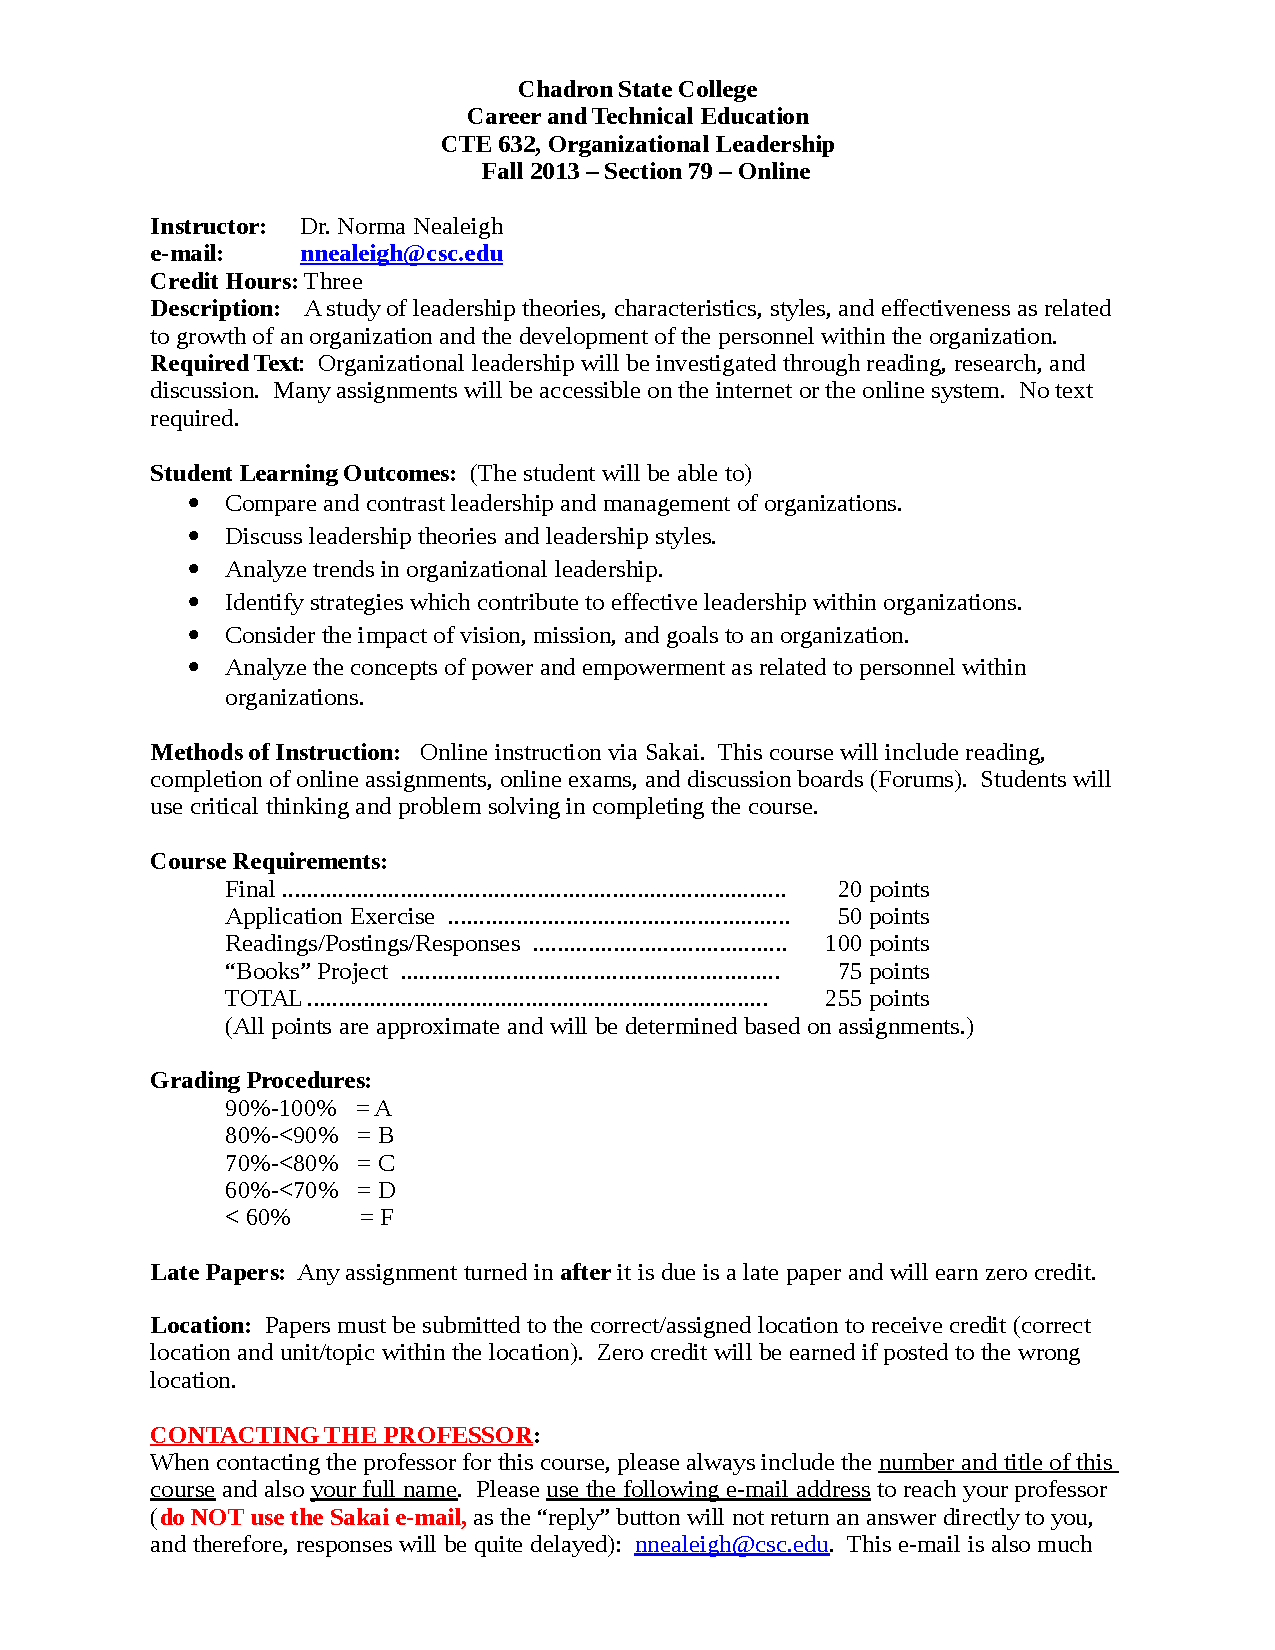
\includepdf[pages=1,pagecommand={\subsubsection{Organizational Leadership Syllabus}}]{CTE632SylbsOnLine139.pdf}
\restoregeometry
\includepdf[pages=2-]{CTE632SylbsOnLine139.pdf}

% Work Examples
\newgeometry{top=.3in}
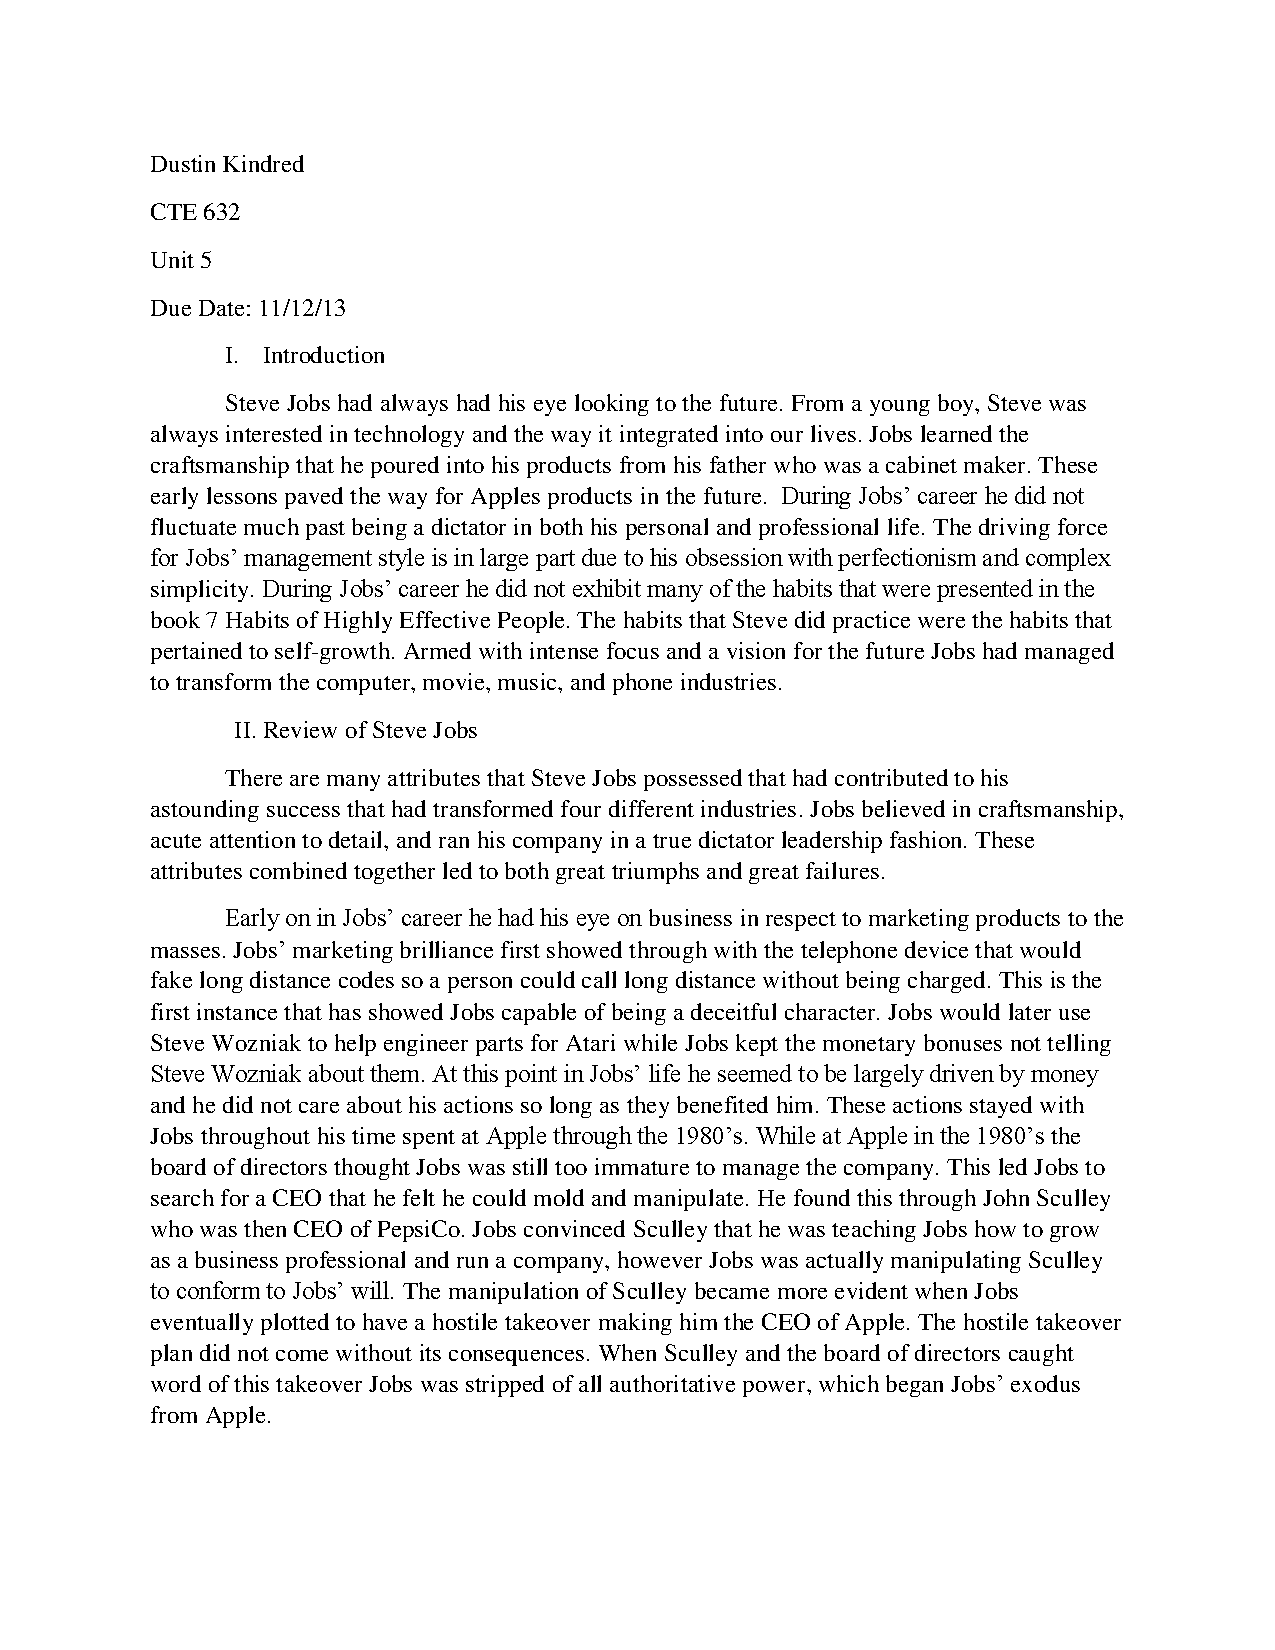
\includepdf[pages=1,pagecommand={\subsubsection{Work Examples}}]{Book_review.pdf}
\restoregeometry
\includepdf[pages=2-]{Book_review.pdf}

% Spring 2014
\subsection{Advanced Behavioral Statistics}
\subsubsection{Reflections}
\paragraph {}
This class used a online format of teaching where are assignments were designed by software including online textbook. I find this format very difficult to interact with and felt that much of the learning was more self learning and not learning from the instructor. Many times when figuring out assignments I would need to seek out other resources to understand the concepts in order to do the homework. This is not the sole fault of the professors teaching, but rather an issue with course work that relies on online software based math courses. Since the course was laid out with software learning this lead to just solving problems without hitting on the course learning outcomes.
\paragraph {}
Throughout the class I did become more familiar with performing ANOVA and CHI Squared tests. Since this course picked-up where my introduction to statistics course left off and I was happy to finish learning some of the more advanced statistical methods. But I did have a hard time grasping the concepts presented in the class and was left wanting more direction in each lesson than the course software provided.
\paragraph {}
What I have taken away from the class is even though I could not recite how to perform some tests today. I do know what types of tests I should be performing in order to arrive at a statistical result. If presented today to perform a statistical analyses I would need to refresh my memory of what is needed in order to give an exact result. I don't feel this is a bad outcome because I am not ignorant to the statistical process.
\newgeometry{top=.3in}
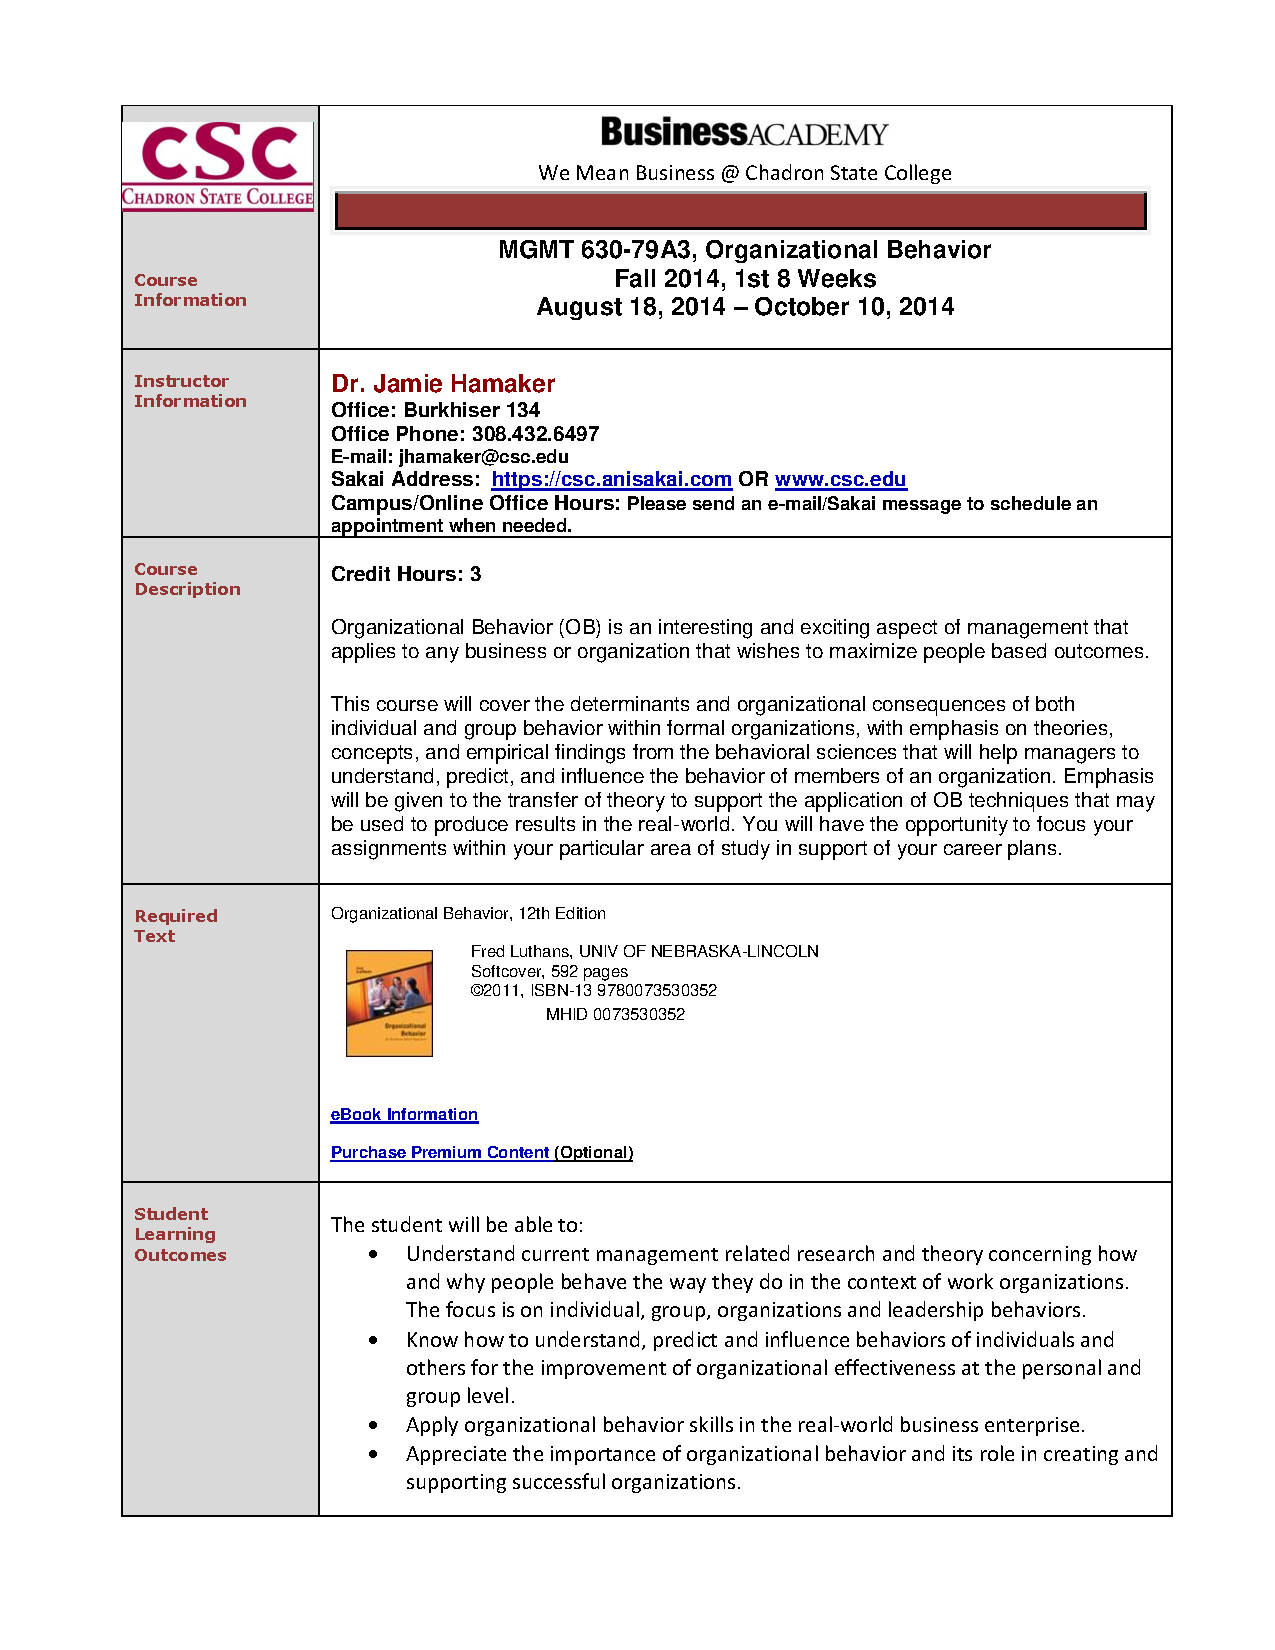
\includepdf[pages=1, pagecommand={\subsection{Advanced Behavioral Stats}}]{Syllabus_MGMT630.pdf}
\restoregeometry
\includepdf[pages=2-]{Syllabus_MGMT630.pdf}

\subsection{Theories of Conflict Resolution}
\subsubsection{Reflections}
\paragraph {}
Conflict Mediation was a hard class for me. Although I use the underlining concepts of this class everyday at work when working with customers. From the moment we started I was wishing the workload would have been lighter. I say this because I felt that the discussion response requirements were so much that the class created an atmosphere of forced response. I understood the purpose of the original in depth discussion. I also understand the purpose of responding to other participants. What I did not understand was the purpose of responding to three other posts with the same in depth response that was required with the original post. I really struggled in writing the in depth responses to three other students and felt that my responses were not genuine and forced as I struggled to meet the requirements of the class. Many times most of the students had close to the same response to the original post which lead to the question of how am I going to write 14 paragraphs three different times explaining how we have a similar experience and perspective. I would have liked to see the requirement for responses limited to “food for thought, insights gained and lessons learned.”
\paragraph {}
From taking this class I have learned that to every decision and every outlook there is a cause for the conflict. Everyone has their own personal perspective and perceives the world differently than the other. Because of varying perspectives we have to work hard to see the world from the other point of view. Once we accomplish this we can work together to create a common ground in which we can work from. The main take away from the class is we all need to take a moment to listen to other and to not speak out of emotion. This is what I understood from the S-TLC system. We must stop then think about what we are listening to then communicate. This acronym can be used just about every conflict from interpersonal to work/co-worker related conflicts.

\newgeometry{top=.3in}
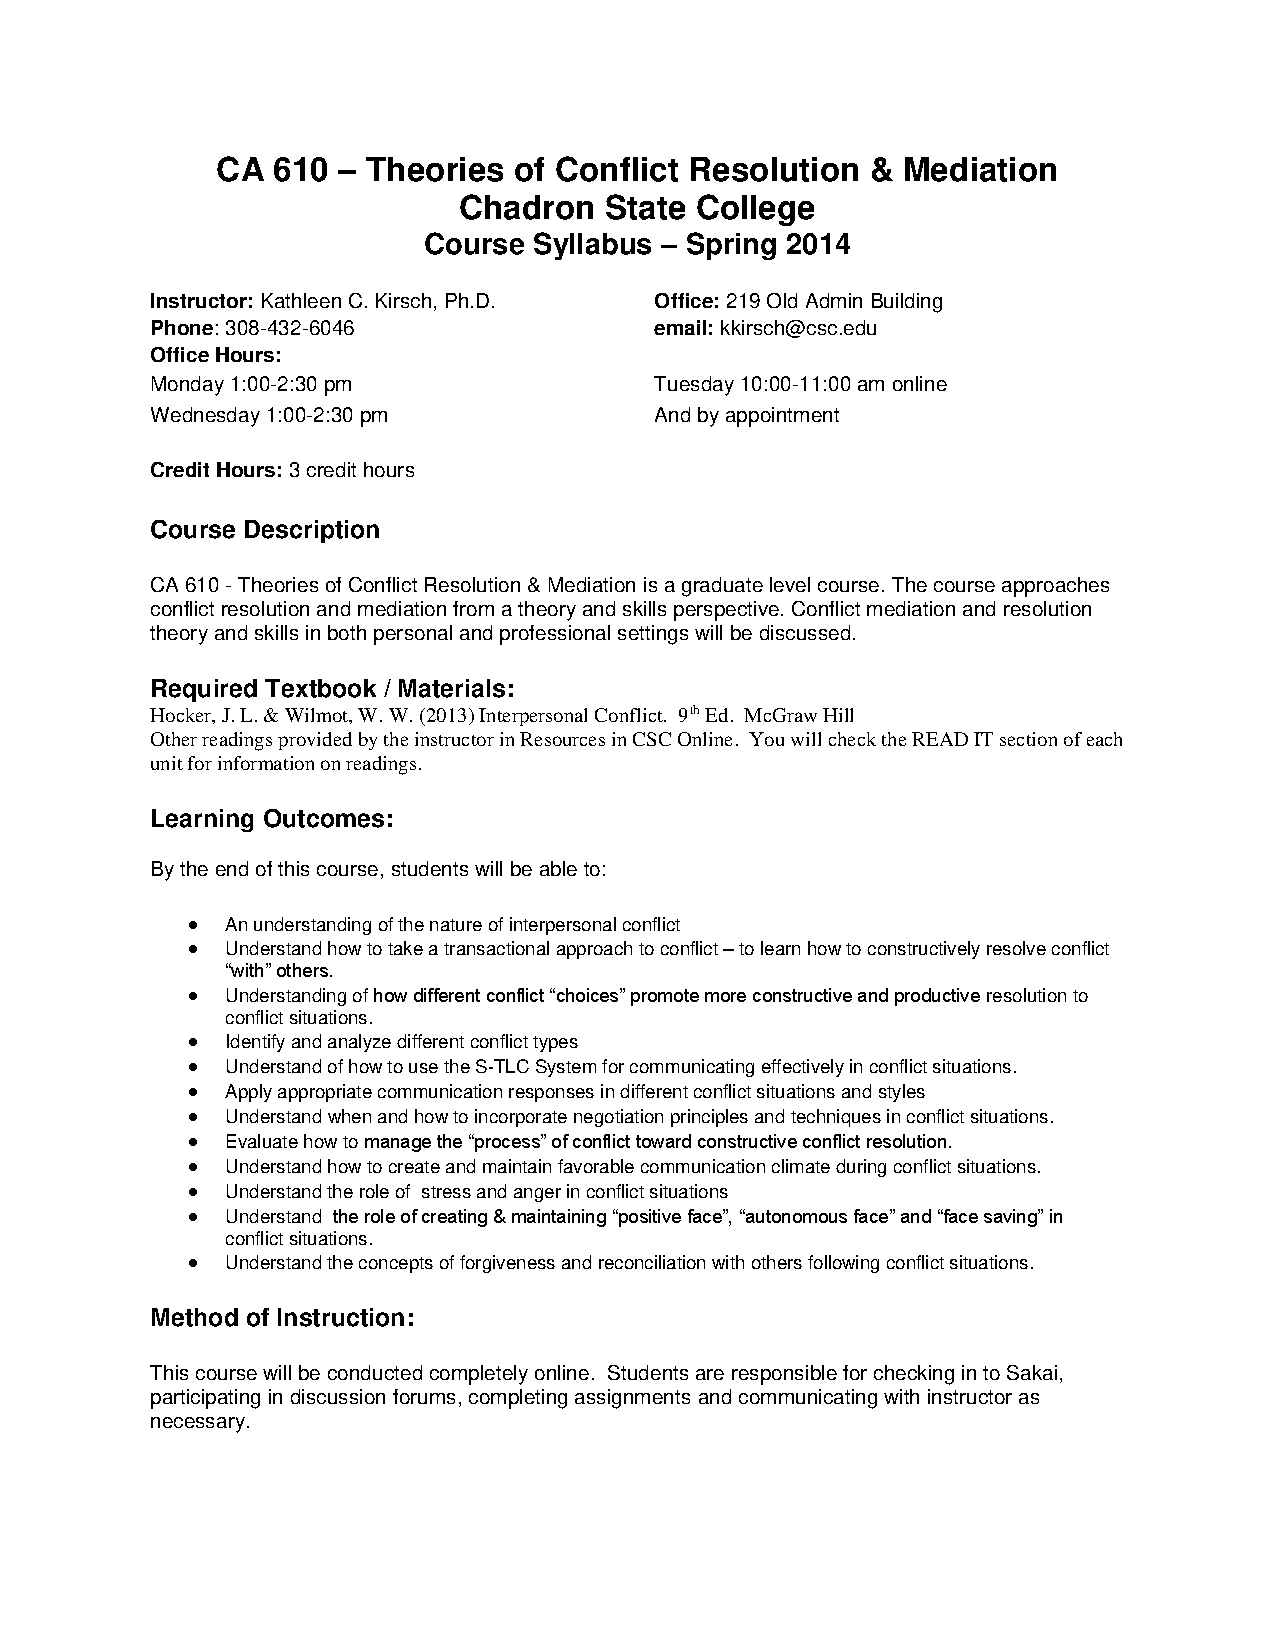
\includepdf[pages=1, pagecommand={\subsubsection{Theories of Conflict Resolution Syllabus}}]{Ca610Spring2014.pdf}
\restoregeometry
\includepdf[pages=2-]{Ca610Spring2014.pdf}
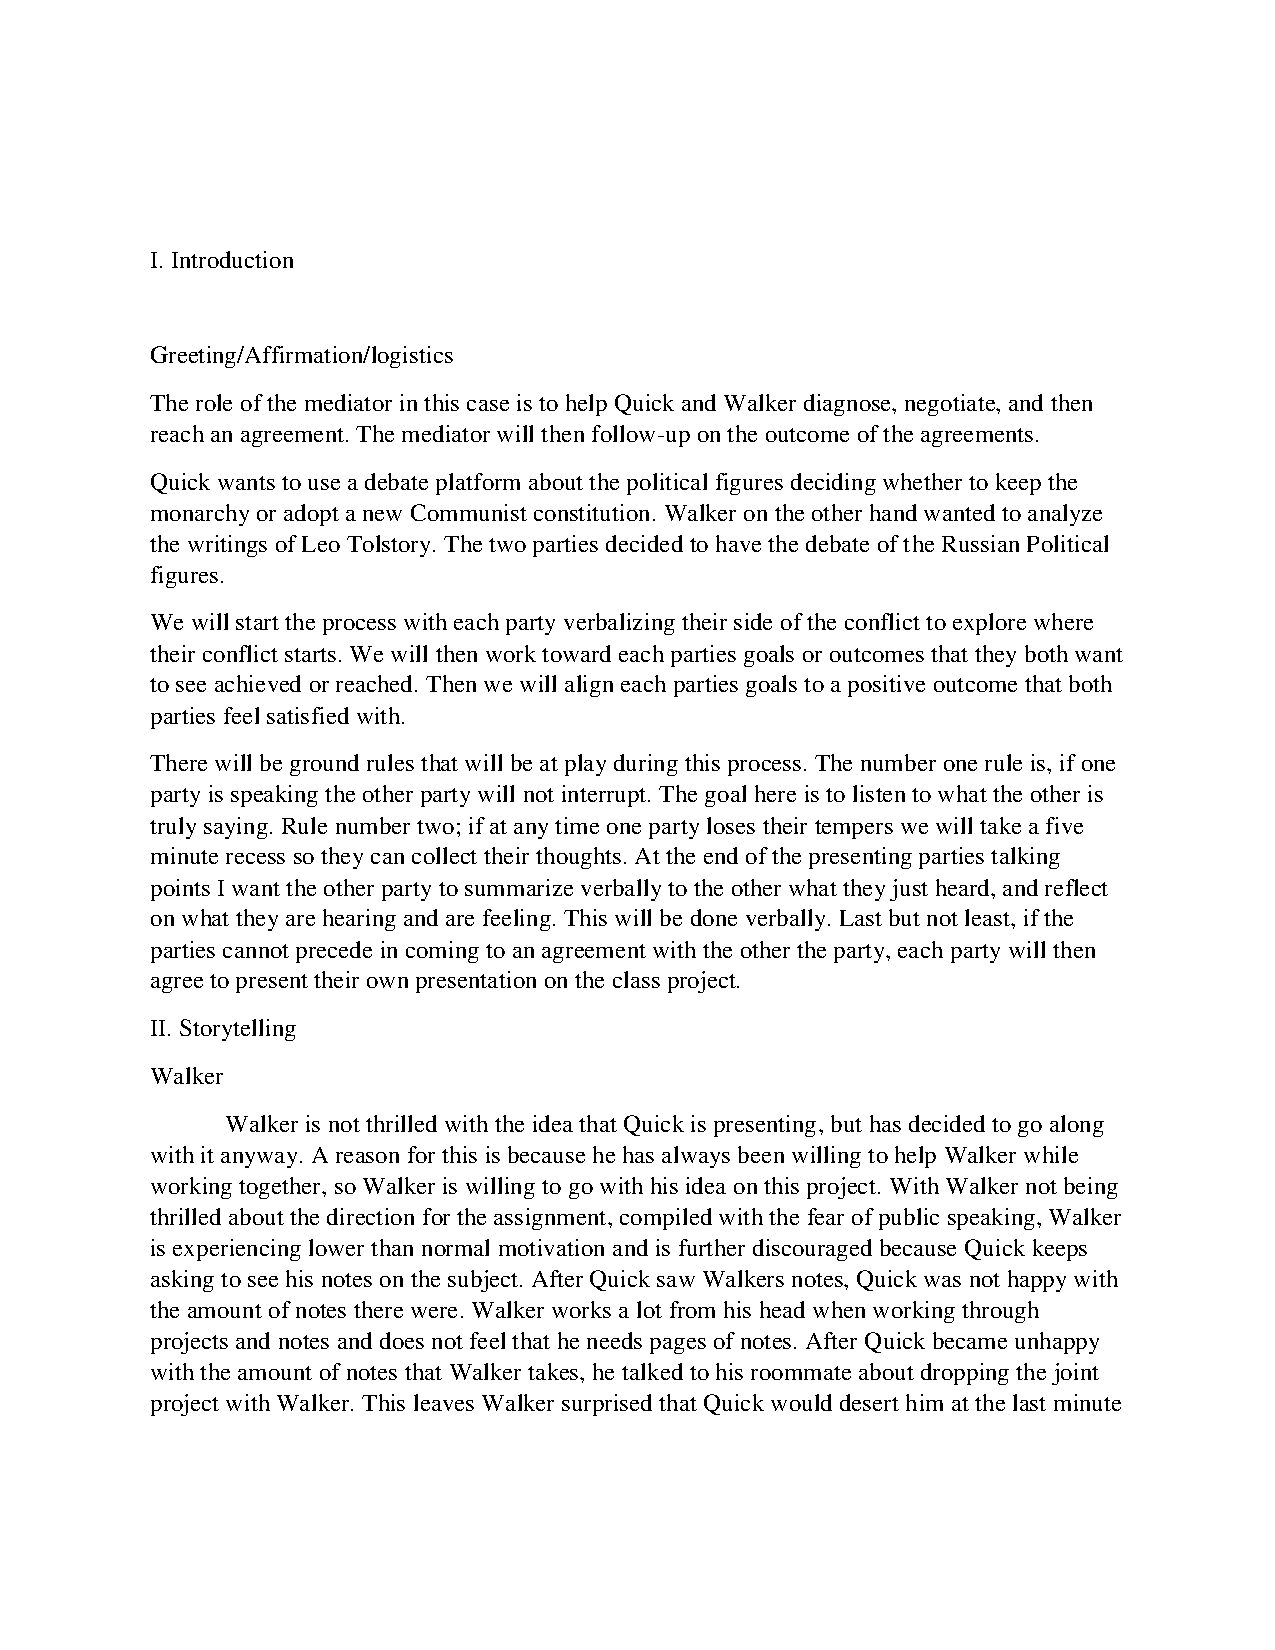
\includepdf[pages=1, pagecommand={\subsubsection{Work Examples}}]{Case_Studies_W-Q.pdf}
\includepdf[pages=2-]{Case_Studies_W-Q.pdf}


% Fall 2014
\subsection{Business Law}
\subsubsection{Reflections}
\paragraph {}
This class should be a required class in any business oriented degree program. I feel that it is so important for everyone to understand legal issues that businesses are presented with everyday. As future leaders we need to stay current with labor regulations environmental regulations and ethical reasoning. Between the text and classroom discussion the class was very interactive with perspectives that ranged from one extreme to the other.
\paragraph {}
I really like the discussions that where included in this class. Dr. Galegos sought out different video or audio clips from different sources such as NPR and various news sites that seemed to be on topic of the readings that week. This was the best way to bridge between traditional classroom teaching and online learning. Every week I looked forward to participating in the discussions because of the relevant material he presented us during the week. On the other side the class assignments were driven to merely provide us with notes for the weekly test. Our assignments were to outline the chapters. For some students this works but does not provide critical thinking needed to fully grasp the many chapters that were assigned weekly. I do understand, however, that the course was a 8 week course with a lot of material that needed to be covered. I just felt that the weekly assignments could have been more meaningful.
\paragraph {}
My undergraduate business law class focused a lot on how to read state statutes, contracts, and how to read court rulings. This class was an extension of that class but focused on regulations nationally and globally. I was not as interested in the chapters which talked about trade regulation and international law as much. This was not because it was poorly described but rather because I have never seen myself in the capacity of international business. The parts of the class I really enjoyed and wanted more of was employee relations and labor management relations and how the regulations work into ethical standards.
\paragraph {}
During and after taking this class I felt that I had grown in relation to how I make organizational decisions. Before these classes thought was not given what legal ramifications exist for each action. The class has really opened my eyes to how we as business leaders need to stay current and possibly develop materials that help other members of the organization to also stay current on regulations and ethical standards as they relate to the type of work we are involved in.
% todo: compile course discussions into one document

\newgeometry{top=.3in}
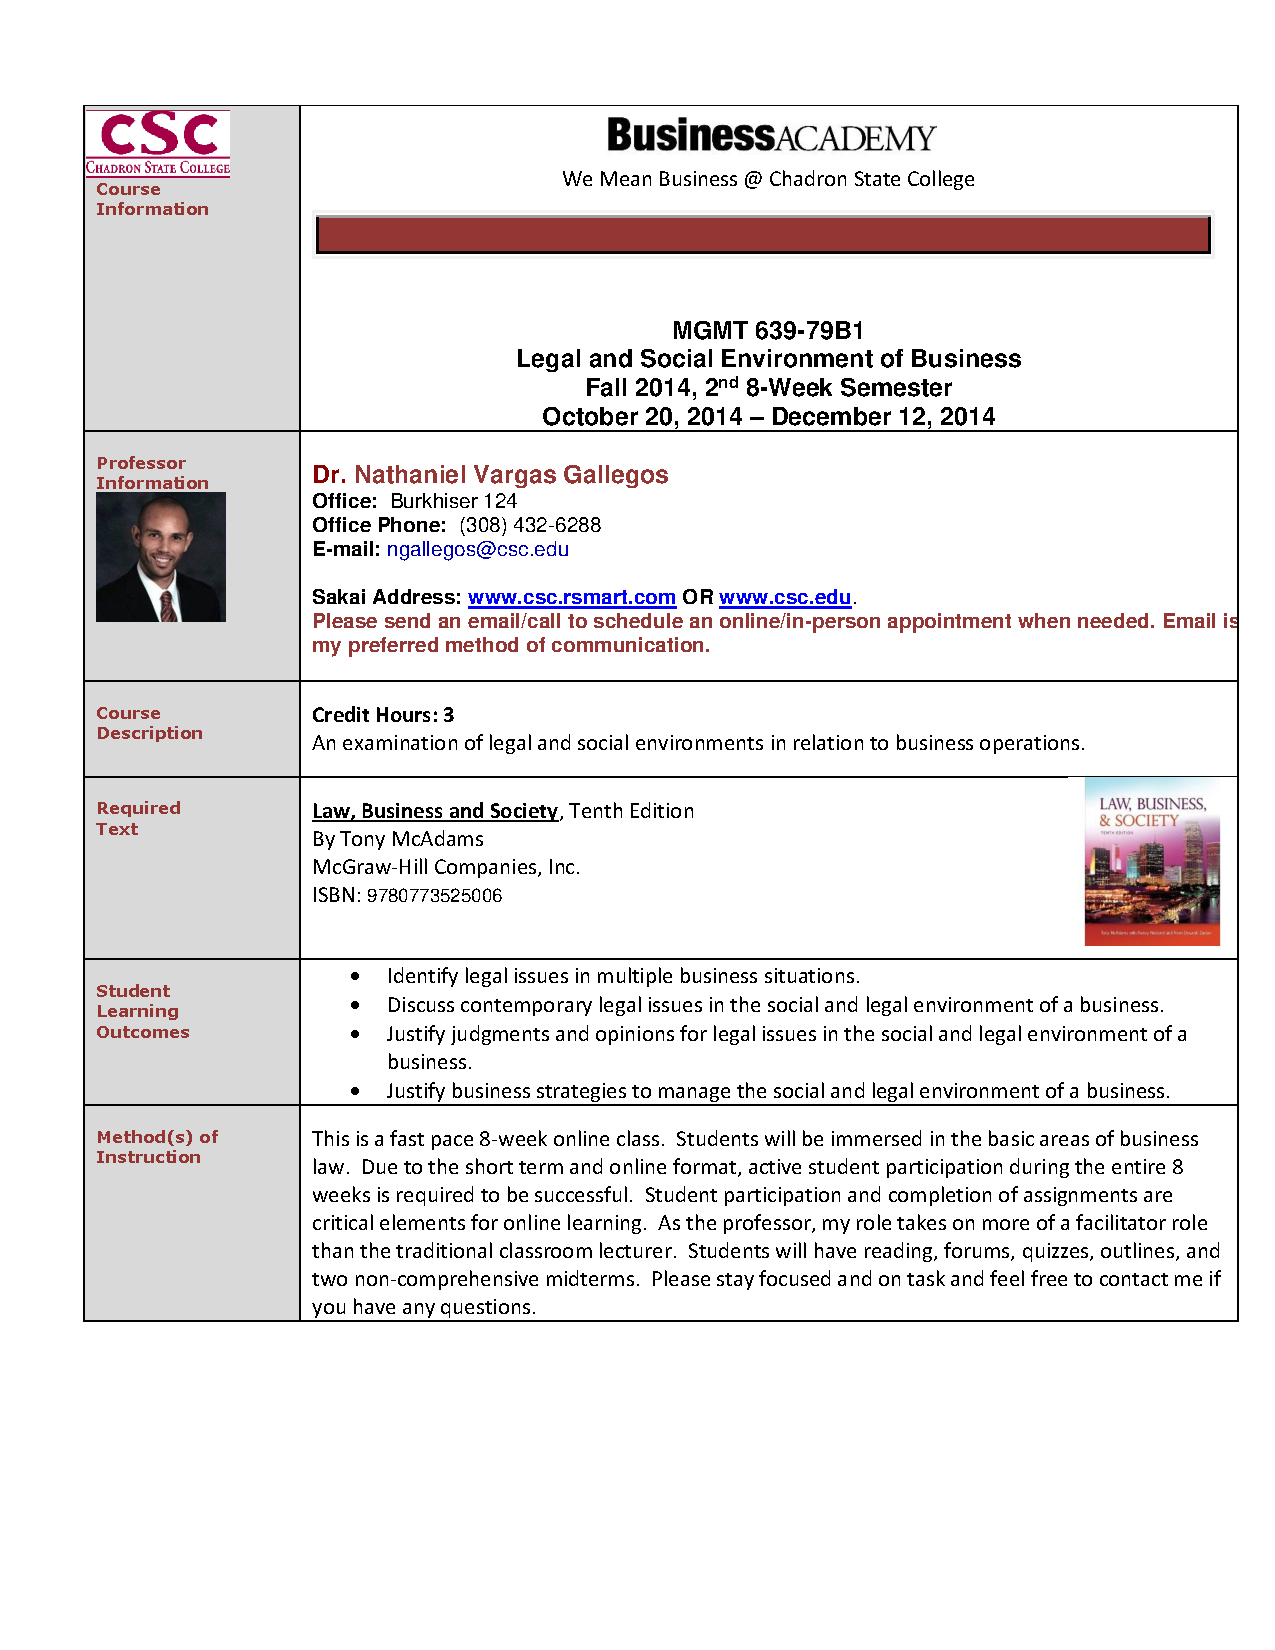
\includepdf[pages=1, pagecommand={\subsubsection{Business law Syllabus}}]{Syllabus_MGMT639-79B1_NGallegos_1148.pdf}
\restoregeometry
\includepdf[pages=2-]{Syllabus_MGMT639-79B1_NGallegos_1148.pdf}

\newgeometry{top=.3in}
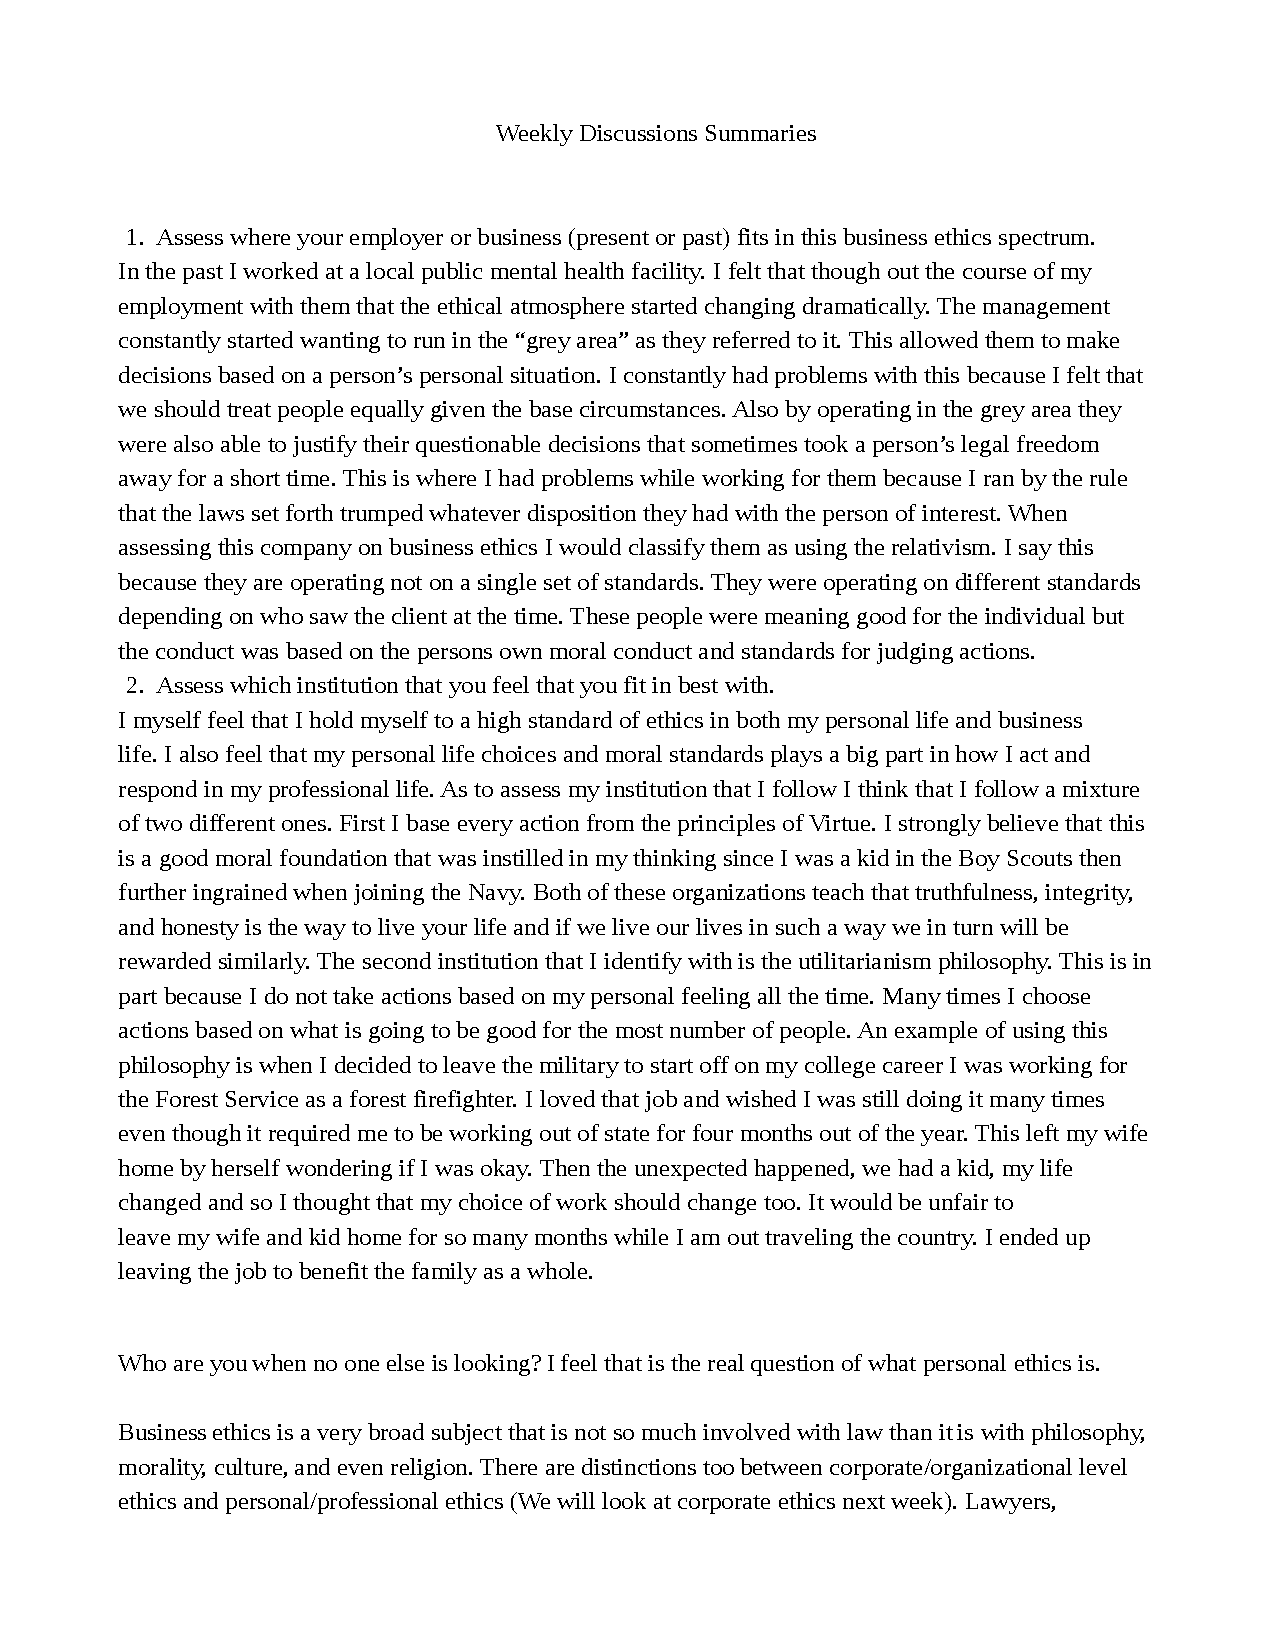
\includepdf[pages=1, pagecommand={\subsubsection{Work Examples}}]{bl_weeklys.pdf}
\restoregeometry
\includepdf[pages=2-]{bl_weeklys.pdf}


\subsection{Organizational Behavior}
\subsubsection{Reflections}
\paragraph {}
I really enjoyed Organizational Behavior because learning how to motivate employees was one of the entire reasons for pursuing this degree path. Starting on this path I was set on the idea that employees make the organization great. This class helped with motivating the workforce to produce the best possible results. One key area was theories of motivation where we learned that monetized incentives only quell employees concerns for a short time but the underlining roots to employee concerns are still there. I find this fascinating because many employers work hard to offer these incentives but they never work on employee relations.
\paragraph {}
During the period of this class we did several company profiles. One profiled American Airlines for corporate culture examples. What we learned is American Airlines is successful because of their corporate culture. The company strives to maintain a fun working environment for their employees. The company also encourages employees at all levels to participate is making work processes better. They also have extensive employee learning opportunities. With everything put together American Airlines have shown the world that when we invest in the workforce the workforce rewards the company with high profit margins with a direct correlation between happy employees and happy customers.
\paragraph {}
Since taking this class I have used different theories described for employee enrichment. One theory that I felt is important was Maslow's hierarchy of needs. Every employer should study this theory and understand the psychological perspectives behind employee motivations. As future leaders we need to understand that we all have the basic needs that needs to be met before we can focus elsewhere. If employers are not supplying living wages to their employees some ramifications could include employees not being motivated to work at their full potential. Other parts of the class that I use is the theory of job enlargement. When employees become proficient in their jobs they need to still be challenged. However job enlargement can be taken to extremes and employees need recognition for the extra duties they have taken on.
\paragraph {}
Overall this class taken with organizational leadership were perfect compliments to each other when learning to become future leaders. The real world examples presented in the class helped with the understanding of how to implement such theories in the workforce. There are plenty of other organizations that we could also model behavior from such as Starbucks or Panera Bread. Teaching the real world examples brought the textbook together driving the point that employees are responsible for making a great company.

\newgeometry{top=.3in}
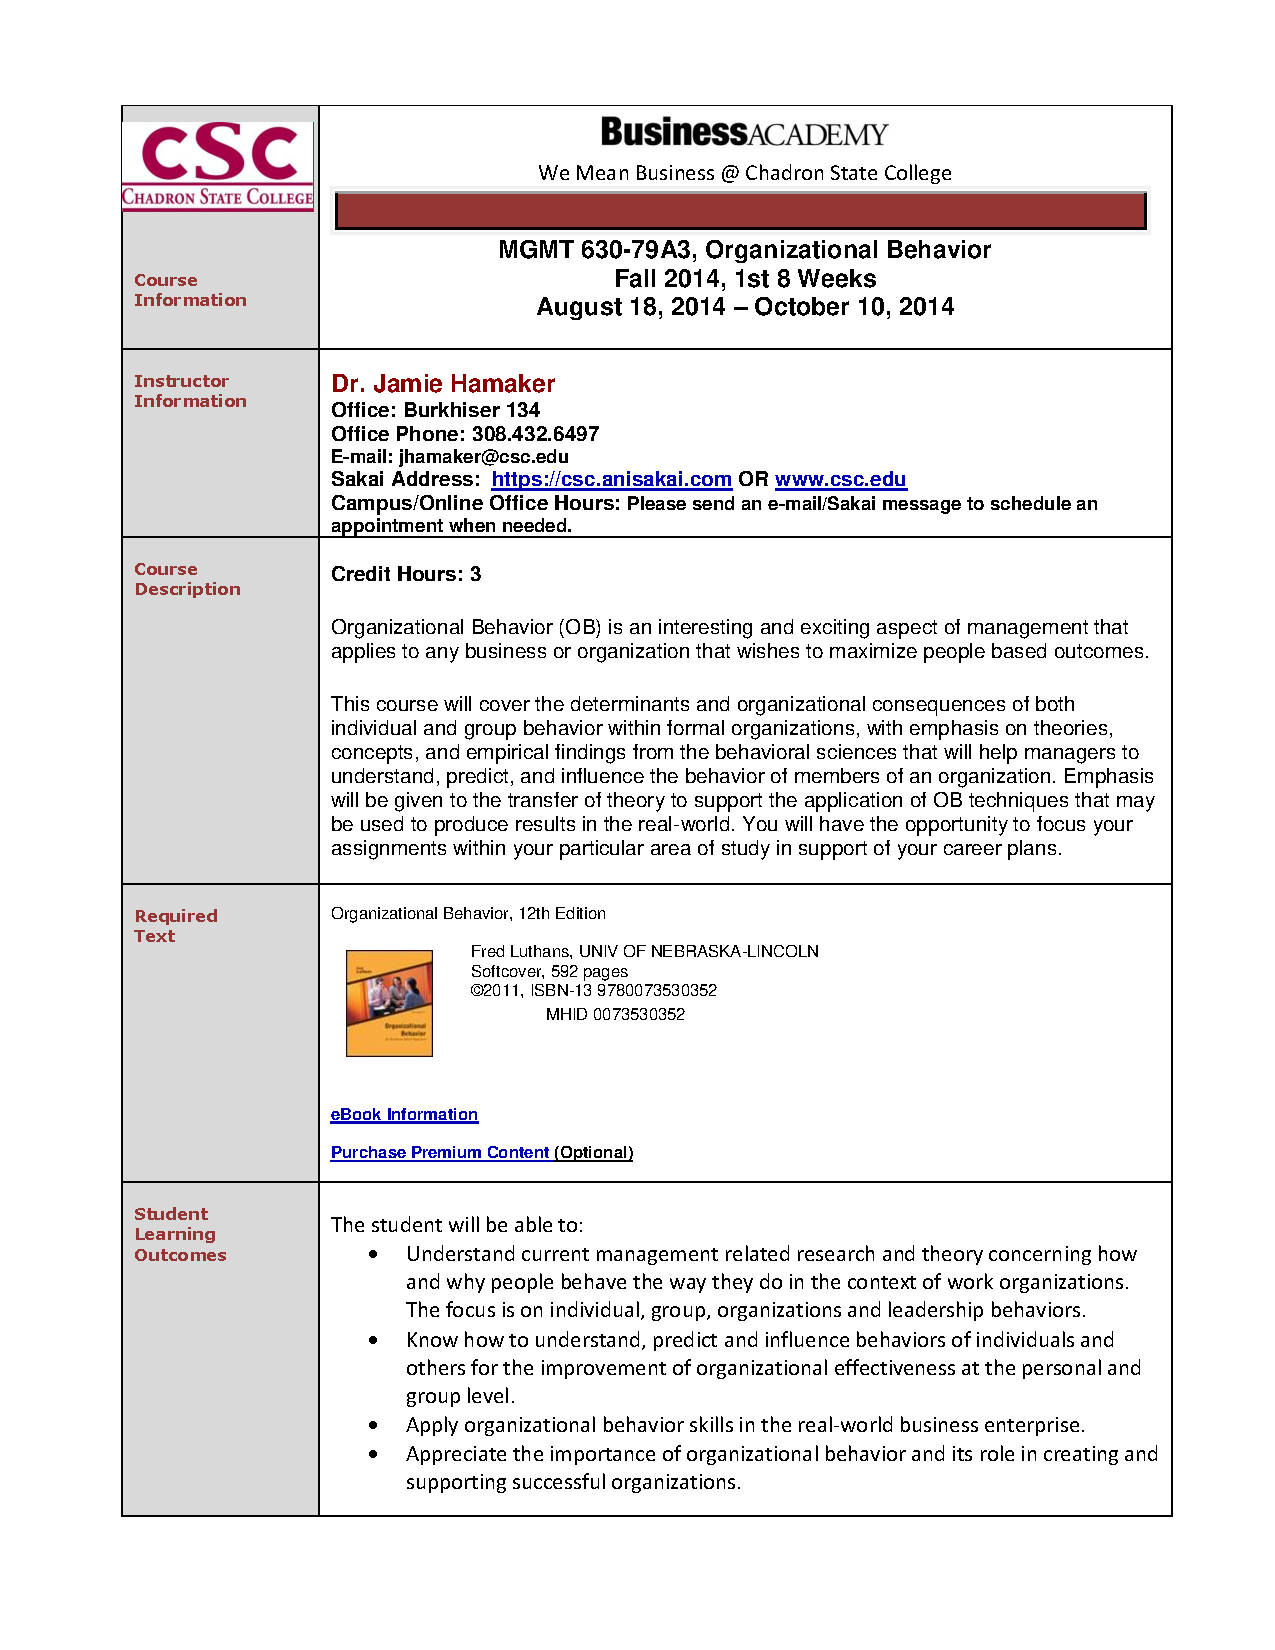
\includepdf[pages=1, pagecommand={\subsubsection{Organizational Behavior Syllabus}}]{Syllabus_MGMT630.pdf}
\restoregeometry
\includepdf[pages=2-]{Syllabus_MGMT630.pdf}
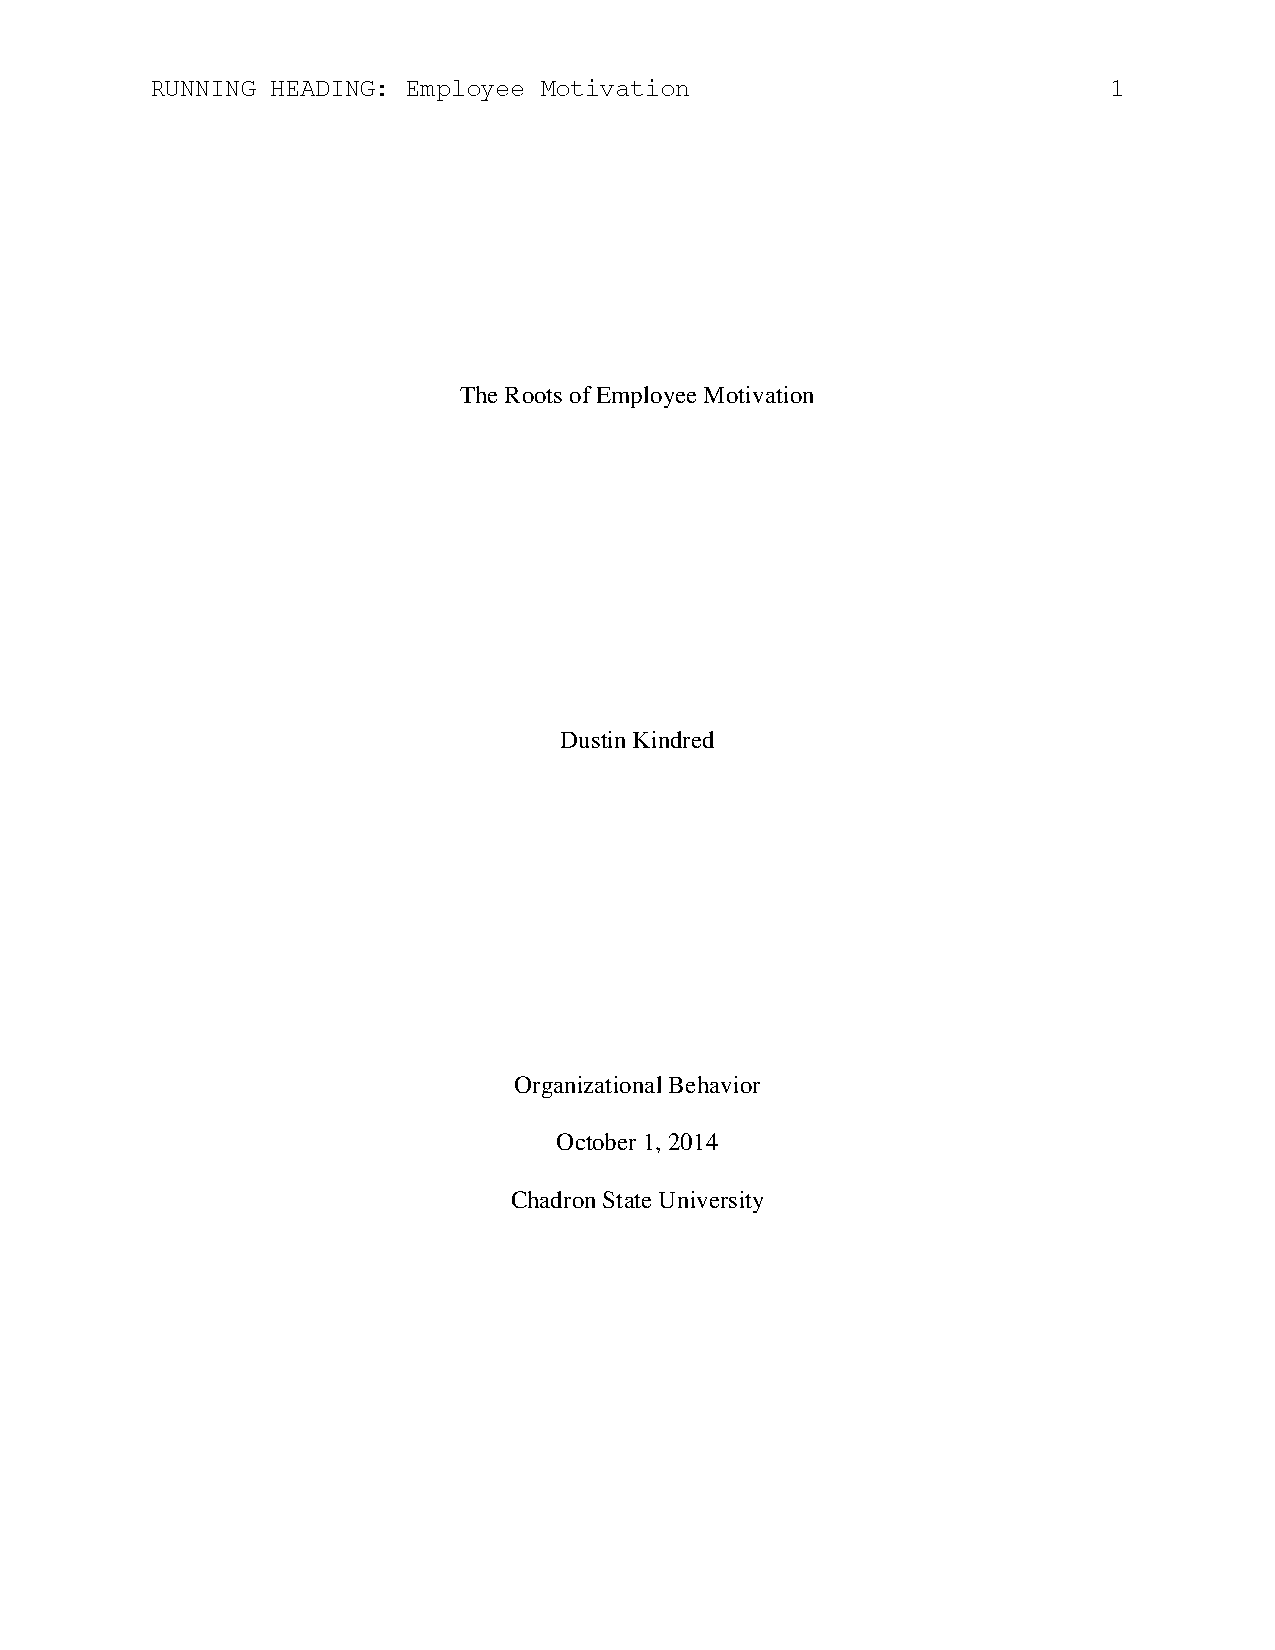
\includepdf[pages=1, pagecommand={\subsubsection{Work Examples}}]{org_behavior_rs.pdf}
\includepdf[pages=2-]{org_behavior_rs.pdf}


% Spring 2015
\subsection{Mathematics for Management}
\subsubsection{Reflections}
\paragraph {}
After taking Mathematics for Management I wasn't sure if I took the same class as the syllabus described. The syllabus describes us demonstrating the principles of compound interest to using discrete random variables using combinatorics. These are the topics that I wanted to learn and was really interested in learning. While participating in the class we had five projects we needed to complete. There were two memorable projects one was a stock market project and the other was a hot dog stand project. The stock market project included us buying and selling stocks and determining profits over the course of a couple of weeks factoring in the cost to buy and sell at certain quantities. The other was starting a hot dog stand and calculating cost of goods as determined from real prices and determining price points to sell our product. The second part of the project was determining an area of our town to sell our product. During this portion we simply needed to record everything we see at this location for a period of time determining if the location is worthy of selling there.
\paragraph {}
At this point I was feeling let down by the course feeling that it was not what I had expected in a class of this level. What I expected was learning the learning outcomes described to also include labor management or budgeting management. Instead the class offered a lesser version of a basic finance class. There were other areas that was challenging to learn. Computing probabilities using normal distribution and discrete random variables in project 3 were challenging. The problems in this section called on the student to find the equation from a data set. This was math I have never learned requiring many hours of research to wrap my head around the concepts. I am still not sure if I fully understand how to arrive at the predictive models. At this point I felt that I should have taken another math class to better understand the concepts in this section and wishing the class had a formal textbook to reference to understand the concepts being described.
\paragraph {}
Overall toward the end of the class we were learning and understanding new math concepts that was a nice departure of stock market exercises. I did wish there was a formal textbook used for the class or at least a school created textbook that fully described the more advanced mathematics. The course was not exactly what I was expecting when I first enrolled but I did learn important concepts such as predictive modeling.

\newgeometry{top=.3in}
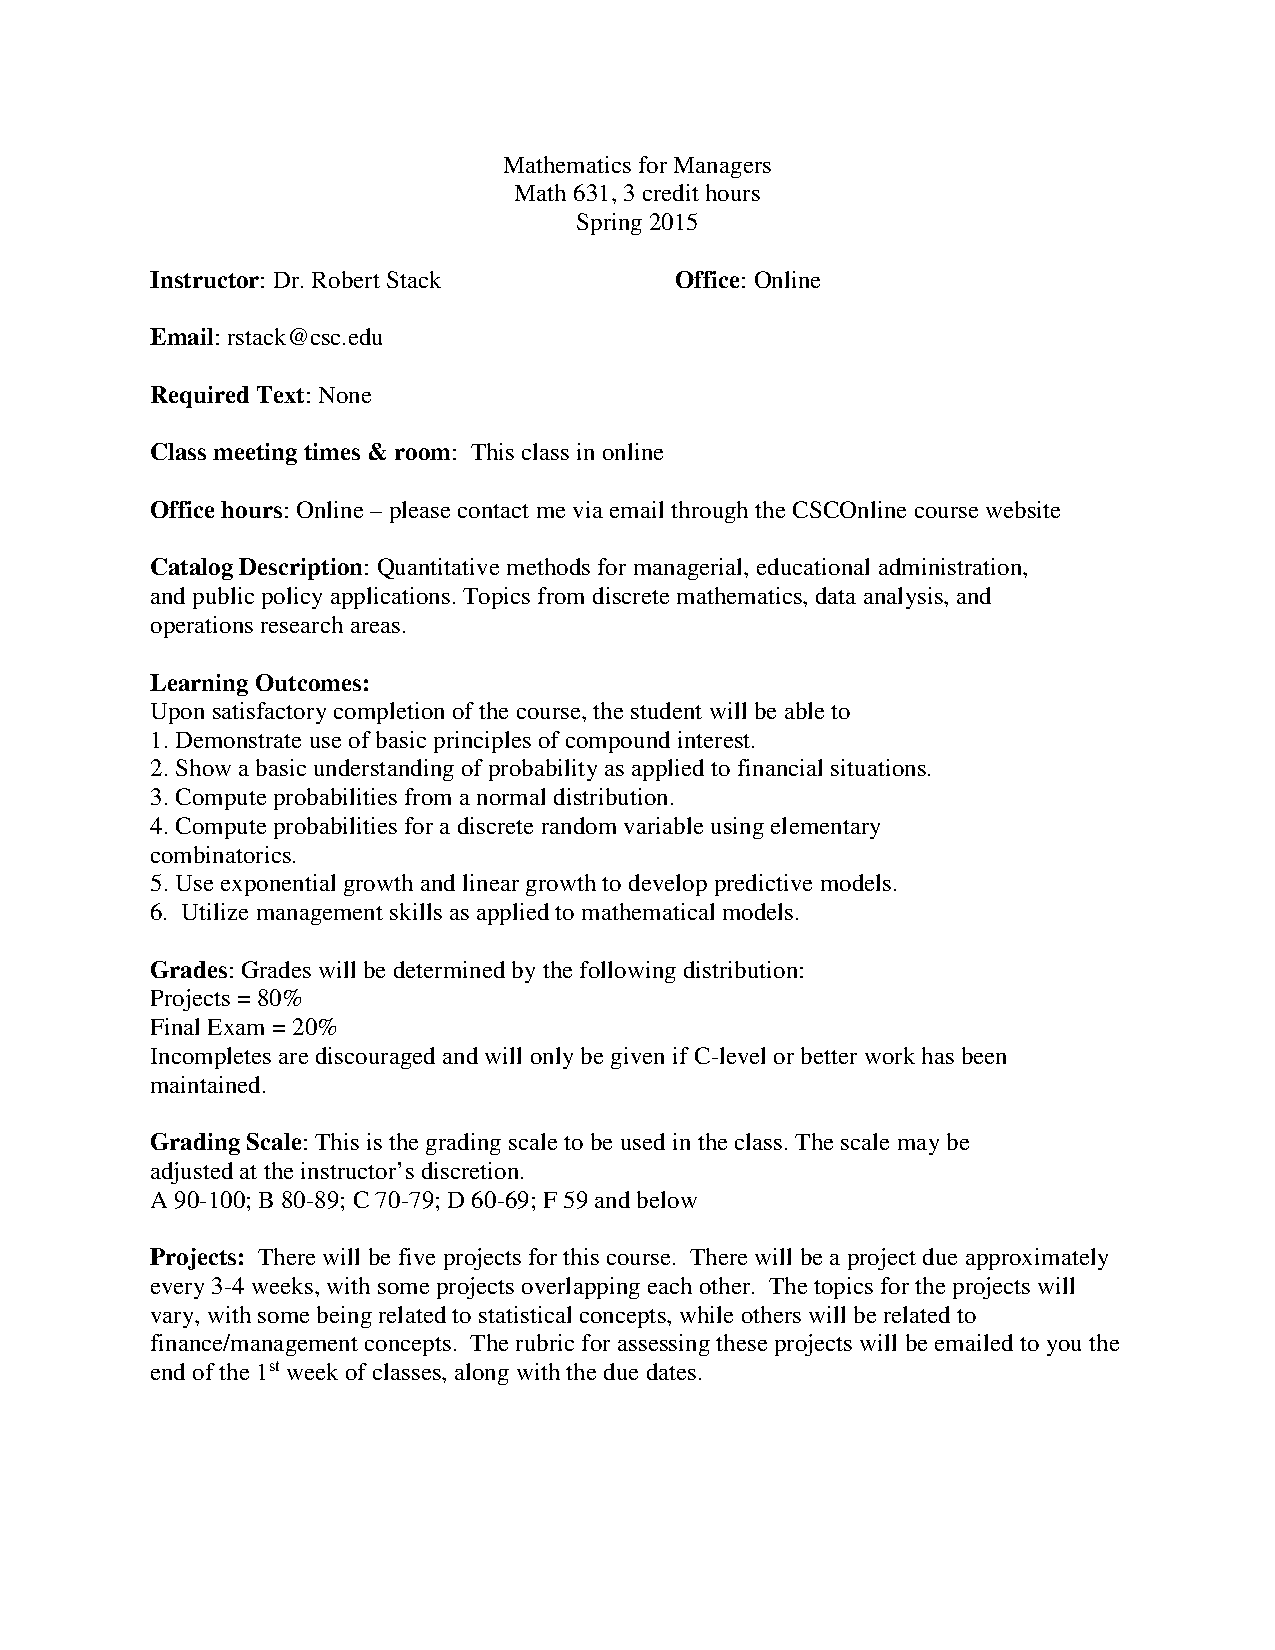
\includepdf[pages=1, pagecommand={\subsubsection{Mathematics for Management Syllabus}}]{Syllabus_MATH631-7901_RStack_1151.pdf}
\restoregeometry
\includepdf[pages=2-]{Syllabus_MATH631-7901_RStack_1151.pdf}

\newgeometry{top=.3in}
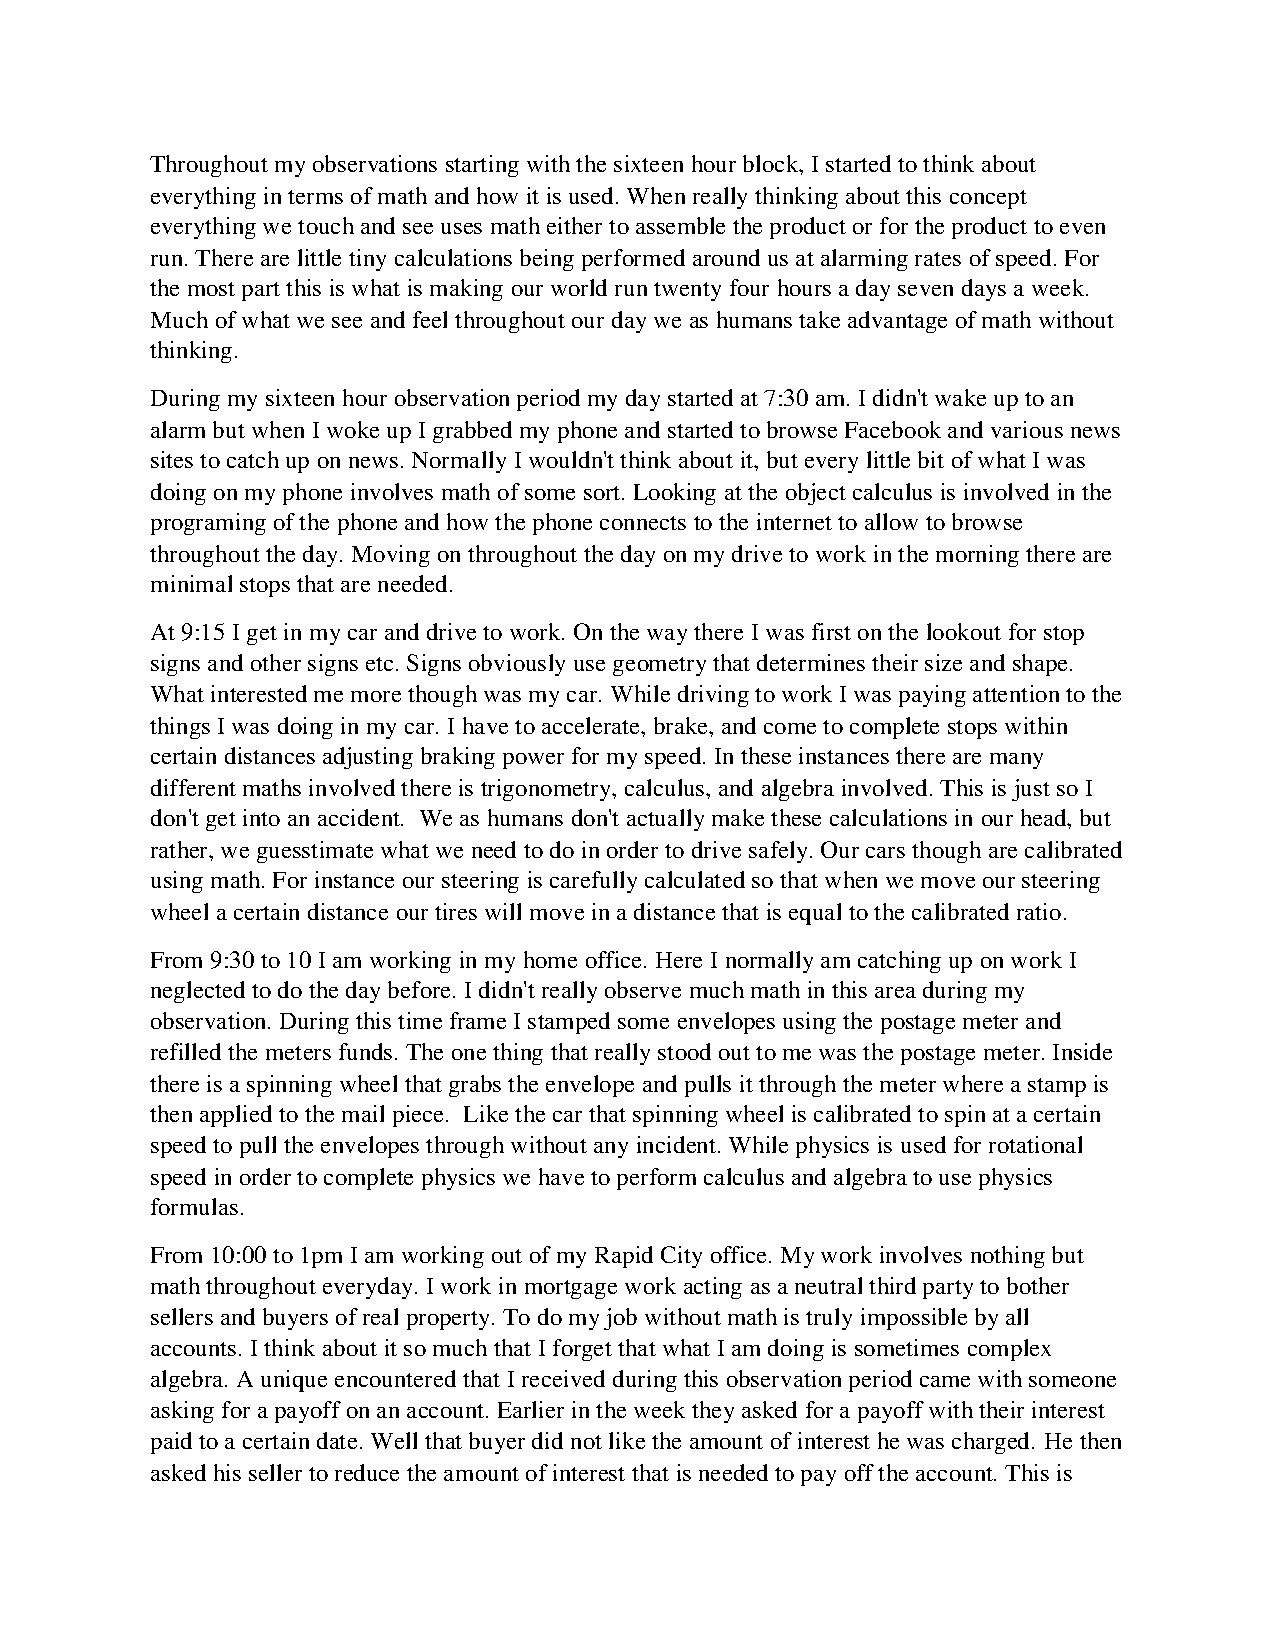
\includepdf[pages=1, pagecommand={\subsubsection{Work Examples}}]{project_4.pdf}
\restoregeometry
\includepdf[pages=2-]{project_4.pdf}


\subsection{Public Relations}
\subsubsection{Reflections}
\paragraph {}
When enrolling in public relations I expected the class to be very dry and boring. Mostly teaching how to interact in public settings, but the class was so much more that this. I enjoyed how public relations played a role with marketing and projecting on organizations image in the public light to influence customer behavior.
\paragraph {}
Throughout the course we learned many concepts that changed our perception of what public relations really is. Before the class my understanding was public relations are centered on press releases and how to handle fallout from company missteps. Though damage control is an important aspect when speaking about this topic, we learned and demonstrated public relations is presenting the company we need to determine how to design our messages to relate the same internally and externally to the public.
\paragraph {}
What I found interesting is how corporate culture can play into how a company is perceived in the publics eye. Everything the company does is considered public relations from ethically sourcing their products to how to handle a product recall. The public looks at these activities when choosing products to buy. Personally as a consumer I look at how the company handles environmental issues. For example I will rarely buy bottled water because of how companies source the water and how environmentally bad this is for local community ground water supply. This ties into public relations because these bottling companies in my eyes have a negative connotation with robbing aquifers. This is what the class has tough me. Everything that can affect employees to the environment affects how the public views the company which ultimately affects their bottom line.
Going forward after taking this course. I now know it's important to know what issues our customers and non-customers feel strongly about. Ultimately the public wants to support a company that acts responsibly both socially and environmentally.
\paragraph {}
The course overall was great. We mixed different media mediums together to develop concrete concepts of effective public relations. After the course was finished I felt that public relations and marketing can work together in the same department. I saw the need for people responsible for public relations to also work close with marketing to ensure the correct messages where presented internally and to the companies publics.

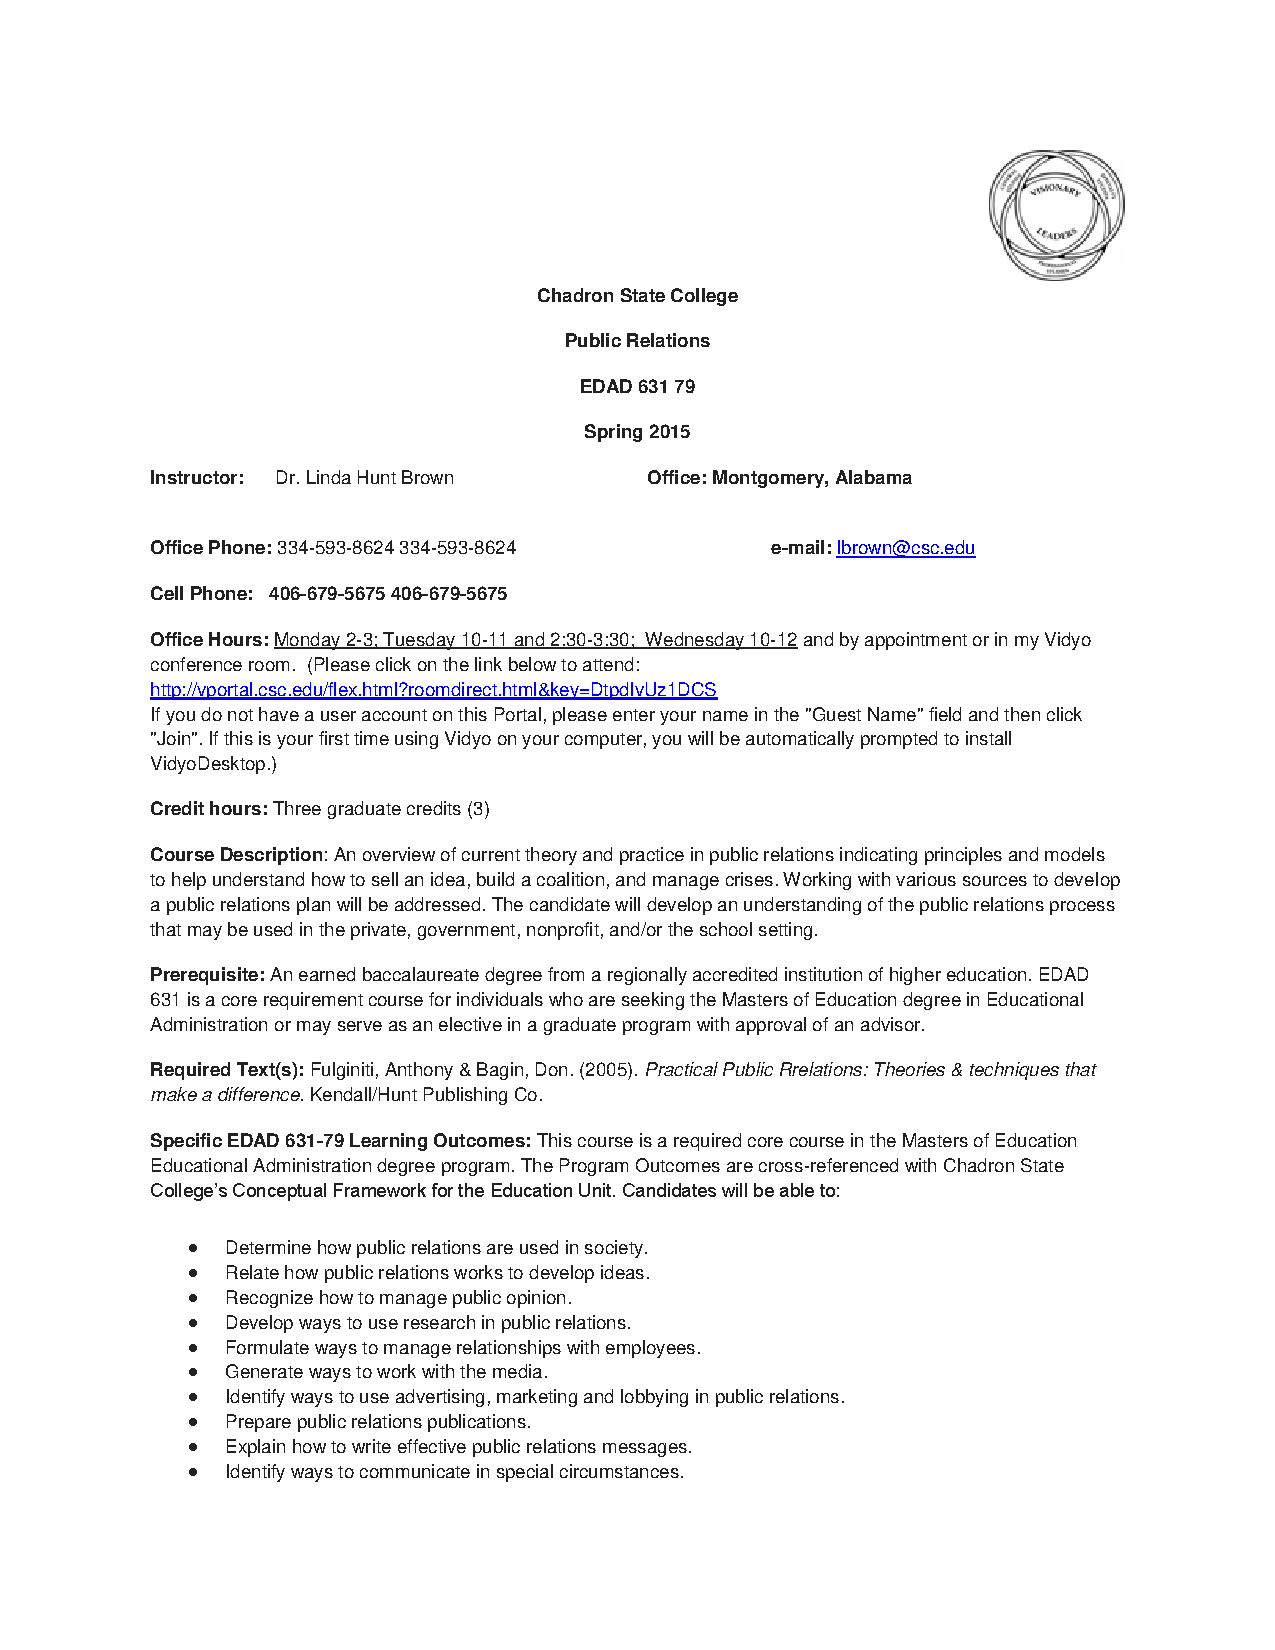
\includepdf[pages=1, pagecommand={\subsubsection{Public Relations Syllabus}}]{Syllabus_EDAD631-7901_LBrown_1151.pdf}
\includepdf[pages=2-]{Syllabus_EDAD631-7901_LBrown_1151.pdf}
\subsubsection{Work Examples}


Please view my work examples at \href{http://www.bit.ly/2eS3K2u}{Dustin's Prezi}



% Fall 2015
\subsection{Human Capital Management}
\subsubsection{Reflections}
\paragraph {}
Human Capital Management was the cornerstone of the degree program. The class was not as easy as I was thinking it was going to be either. The reason why I chose the human resources degree path is because I have worked in both great and poor organizations when taking about how employees were taken care off. What I have witnessed first hand is that when an organization has a great human capital plan that extends further than the human resources department the company as a whole tends to do great things. This is an important observation because my theorized slogan states that the organization does not make the company great but rather the people make the organization great. When we learn how to effective acquire great talent then learn how to retain that talent the company is doing a great job. This leads to the why I looked forward to this class which summed the culmination of the entire degree program. I wanted to better understand job design, recruiting, training programs, performance appraisals and so on.
\paragraph {}
The class presented us with what our expectations where. We quickly designed jobs and created training programs used in an organization that included a variety of different training methods. Perhaps one of the more eye opening exercises was learning and creating benefits packages for a fictitious company. I also really enjoyed the group projects of learning about human capital management of a real company. My group during one group project choose to profile Starbucks. I think this is where some of the most enlightened insights of the class came. While Interviewing a local Starbucks store manager I found myself asking several questions about how the human resources department deals with the management of thousands of employees in different areas of the country at once. What I had learned is that Starbucks does take really good care of their employees, however, there is a disconnect on the local levels of how to perform certain functions such as recruitment and employee appraisals.
\paragraph {}
Though I don't think that I will ever be in a position where I am working in a large corporation running a HR department that is responsible for every location. I know that if I were in the position I would make it a priority of the HR department to work with the locations to meet their needs and demographics.
\paragraph {}
What I truly learned was from personal experience employees have a negative view of the HR department. This perception should not exist since the department and the HR professional job are literally created to benefit the employees. From the teaching of the course the HR department should be a treasured department of the employees. If this is not the case then we need to re-evaluate how to become effective with the workforce. The re-evaluation comes from job design and analysis, providing fair and effective performance reviews and administering compensation packages that get the workforce motivated.

\newgeometry{top=.3in}
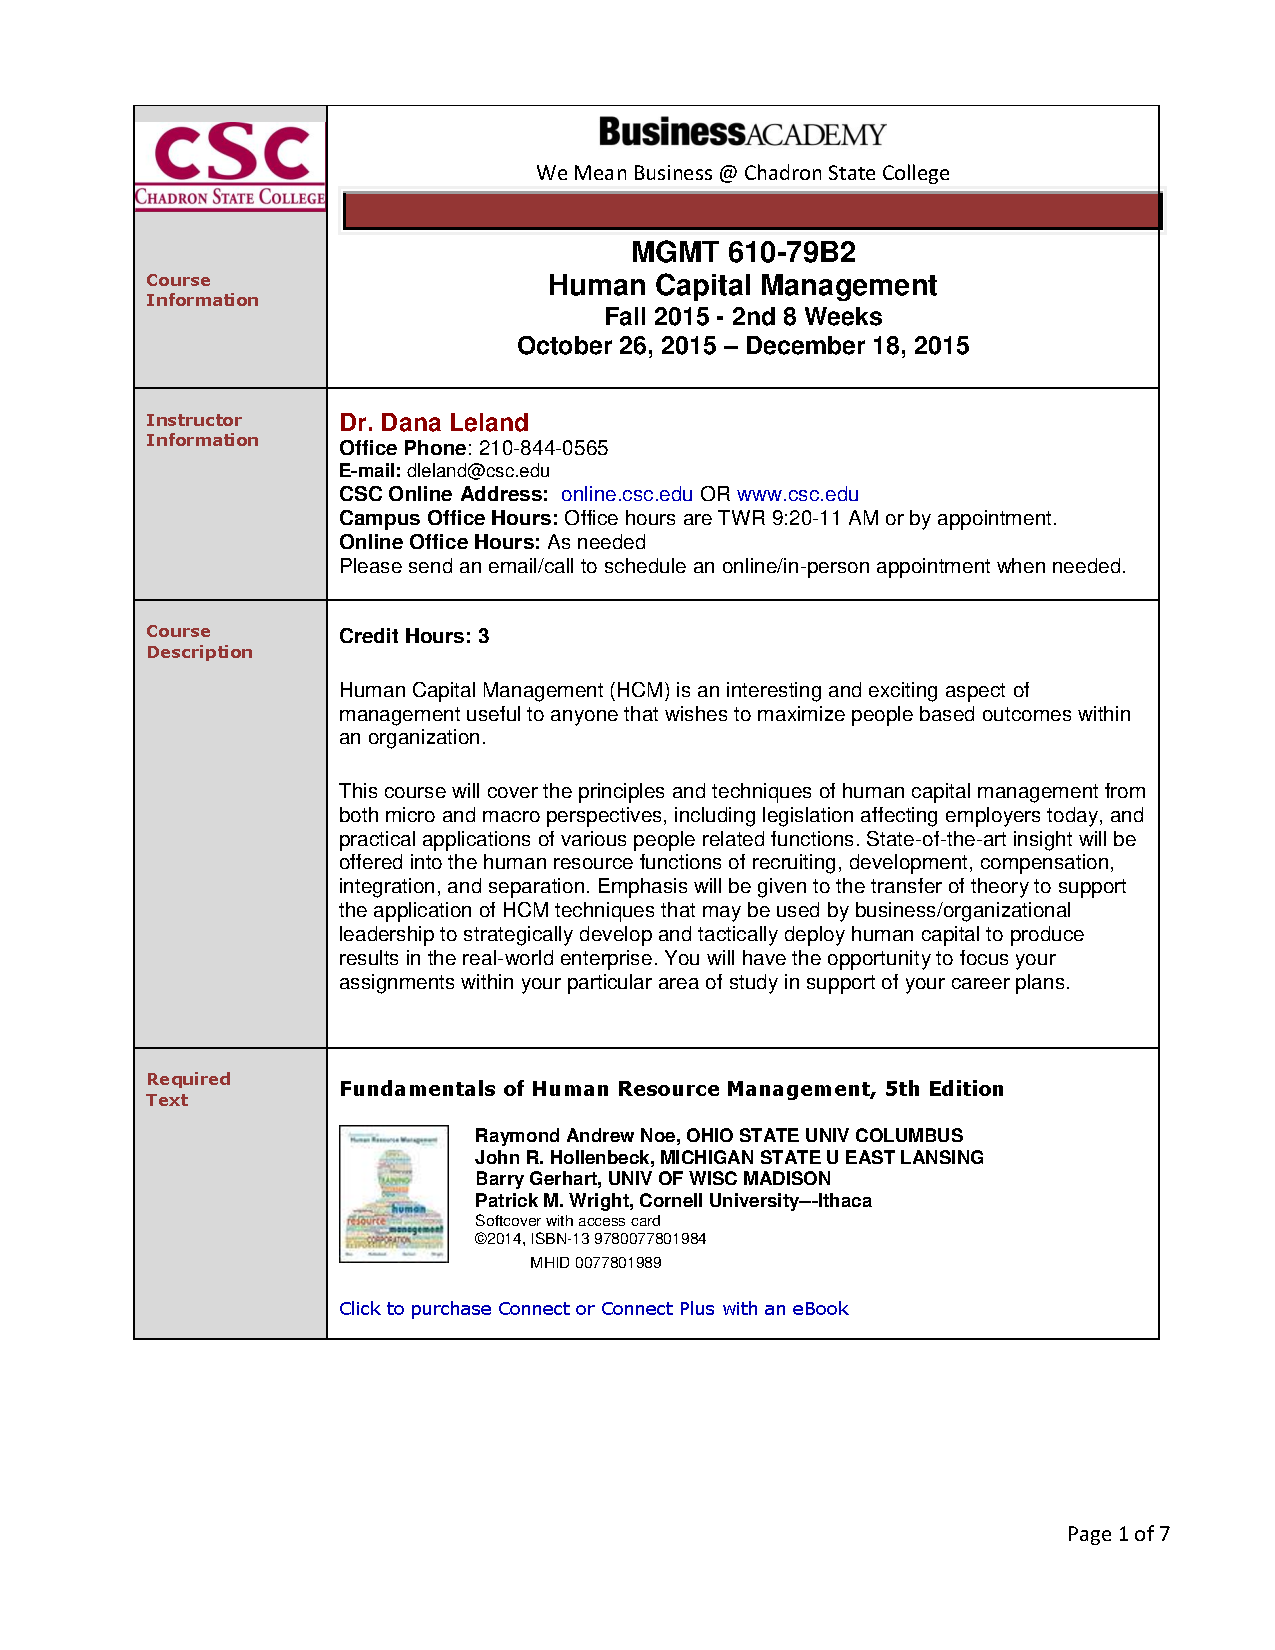
\includepdf[pages=1, pagecommand={\subsubsection{Human Capital Management Syllabus}}]{Syllabus_MGMT610-79B2_DLeland_1158.pdf}
\restoregeometry
\includepdf[pages=2-]{Syllabus_MGMT610-79B2_DLeland_1158.pdf}
\newgeometry{top=.3in}

\includepdf[pages=1, pagecommand={\subsubsection{Work Examples}}]{hcp_rp.pdf}
\restoregeometry

\includepdf[pages=2-]{hcp_rp.pdf}
% todo: Need Syllabus

\subsection{Marketing Management}
\subsubsection{Reflections}
\paragraph {}
It is most likely my expectations but I am always let down by marketing classes. When enrolling in these classes I am always expecting to learn the creative aspects of marketing. I want to learn different marketing messages. I want to leave the class knowing how to market creatively. Marketing Management was no exception to my perceived thought process of what I wanted to learn versus what the class actually was. Mr. Benson did a wonderful job of presenting the material that was contained in our textbooks and I really enjoyed the ongoing assignment and simulation the class presented. In fact I wish more courses or textbook companies would figure out how to create simulations for other courses as well. I respond really well to the quasi real world teaching of the textbook material.
\paragraph {}
The particular simulation the we had was a pharmaceutical company. Each week we competed against each other to become the best company based on our weekly decisions to introduce new products and invest in marketing in different ways. That makes it a great activity that pairs well with other course materials.
\paragraph {}
This course has taught me that marketing is not just advertising. Marketing is a wide variety of activities from researching price points, when to introduce new products and how to perform market research. Market research probably is one of the most important aspects of the marketing process. Without the research the organization in flying blind into an ocean of products and services without knowing what the demand is or what their market segments are. Simply, it is not enough to have an inventive advertising campaign. We need to direct our marketing efforts based on the market segment we are trying to reach. This would involve creating different images depending on the part of the world or country we want to reach.
\paragraph {}
Marketing Management has caused me to really start thinking about where and how to direct efforts of customer acquisition. To start I need to know what are the different markets for a product and what are the different needs for each market. I think I am now better poised for these different analyses now than before. I realize that one class isn't making us an expert on the topics but the fundamentals are there creating pivotal points in the future.
\paragraph {}
In sum I may never find the class or coursework that I am looking for relating to marketing most likely because I have the wrong view of what marketing is. This class has helped shape my views of how to best position a organization to maintain a healthy bottom line while maintaining high ethical standards. My only wish is that I would have taken this class at the same time as public relations because these two would have worked nicely together.

\newgeometry{top=.3in}
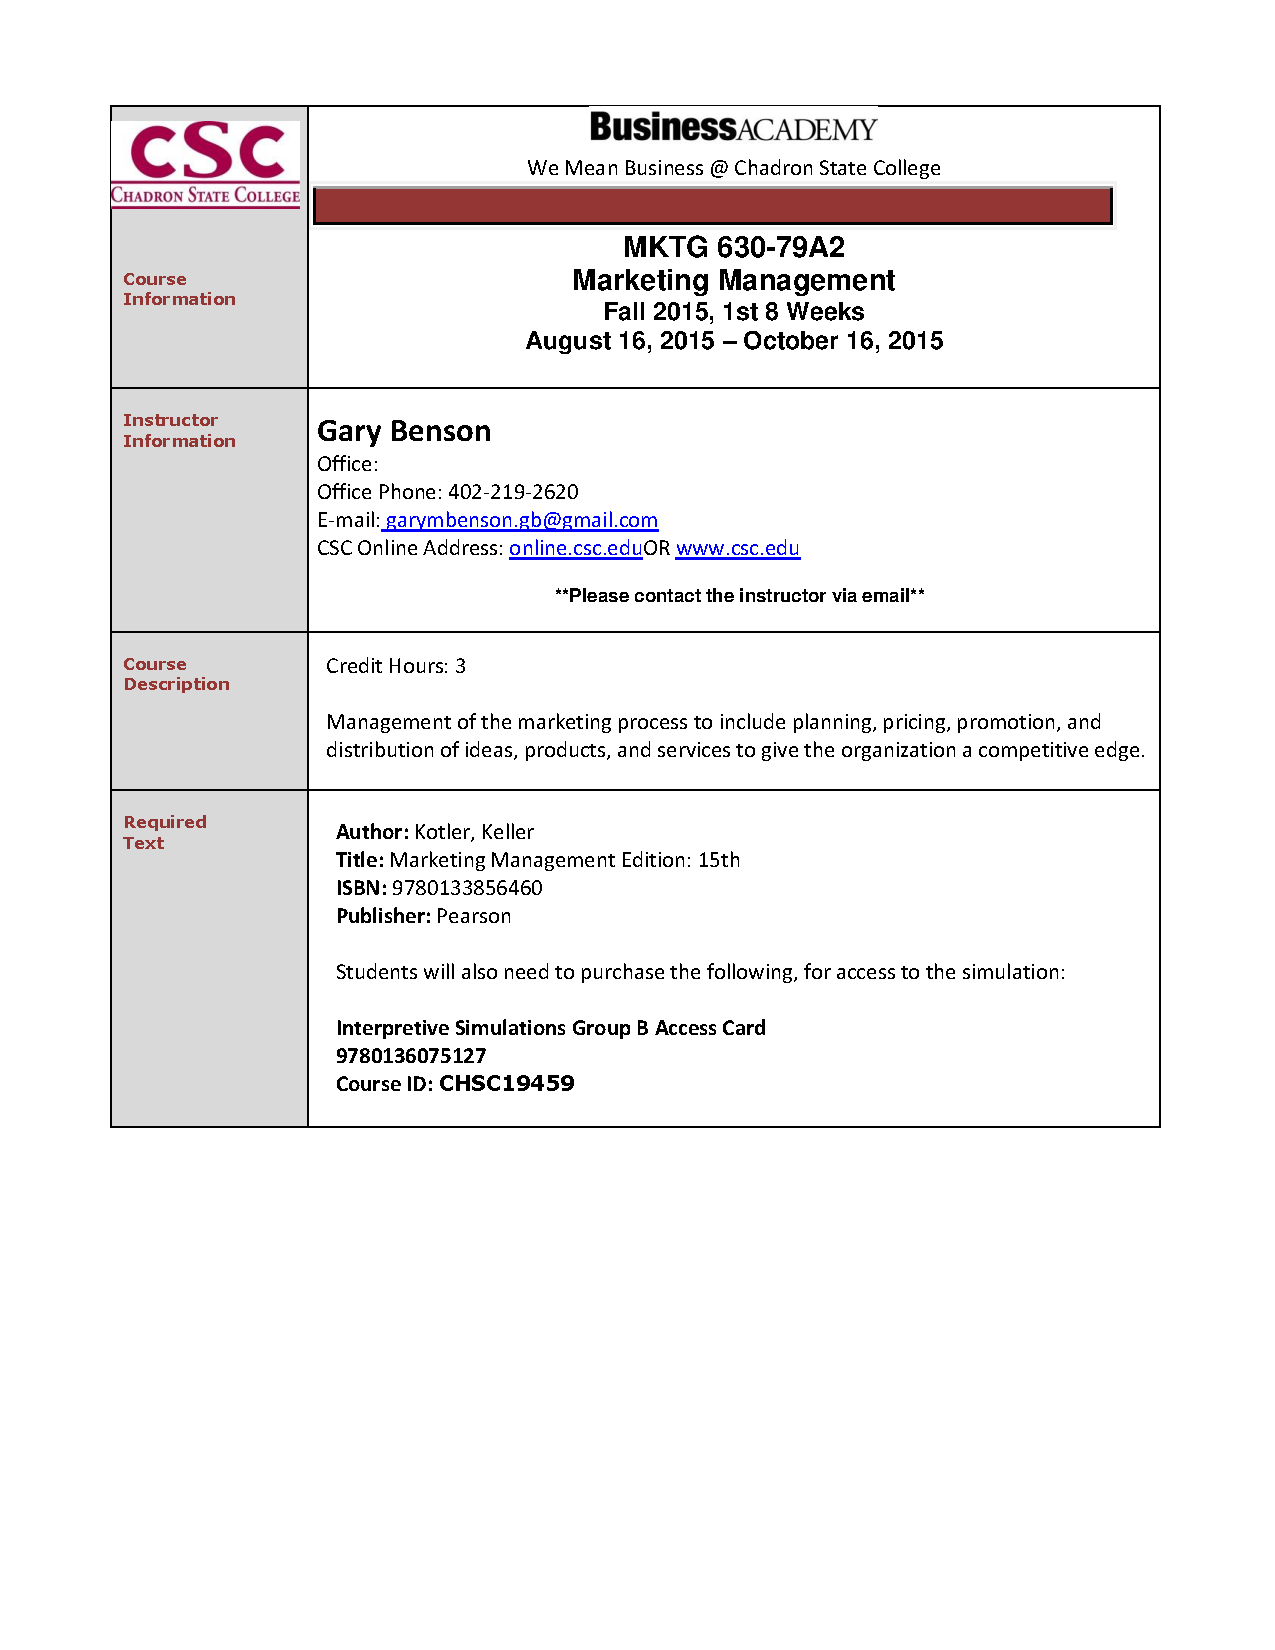
\includepdf[pages=1, pagecommand={\subsubsection{Marketing Management Syllabus}}]{Syllabus_MKTG630-79A2_GBenson_1158.pdf}
\restoregeometry
\includepdf[pages=2-]{Syllabus_MKTG630-79A2_GBenson_1158.pdf}

\newgeometry{top=.3in}
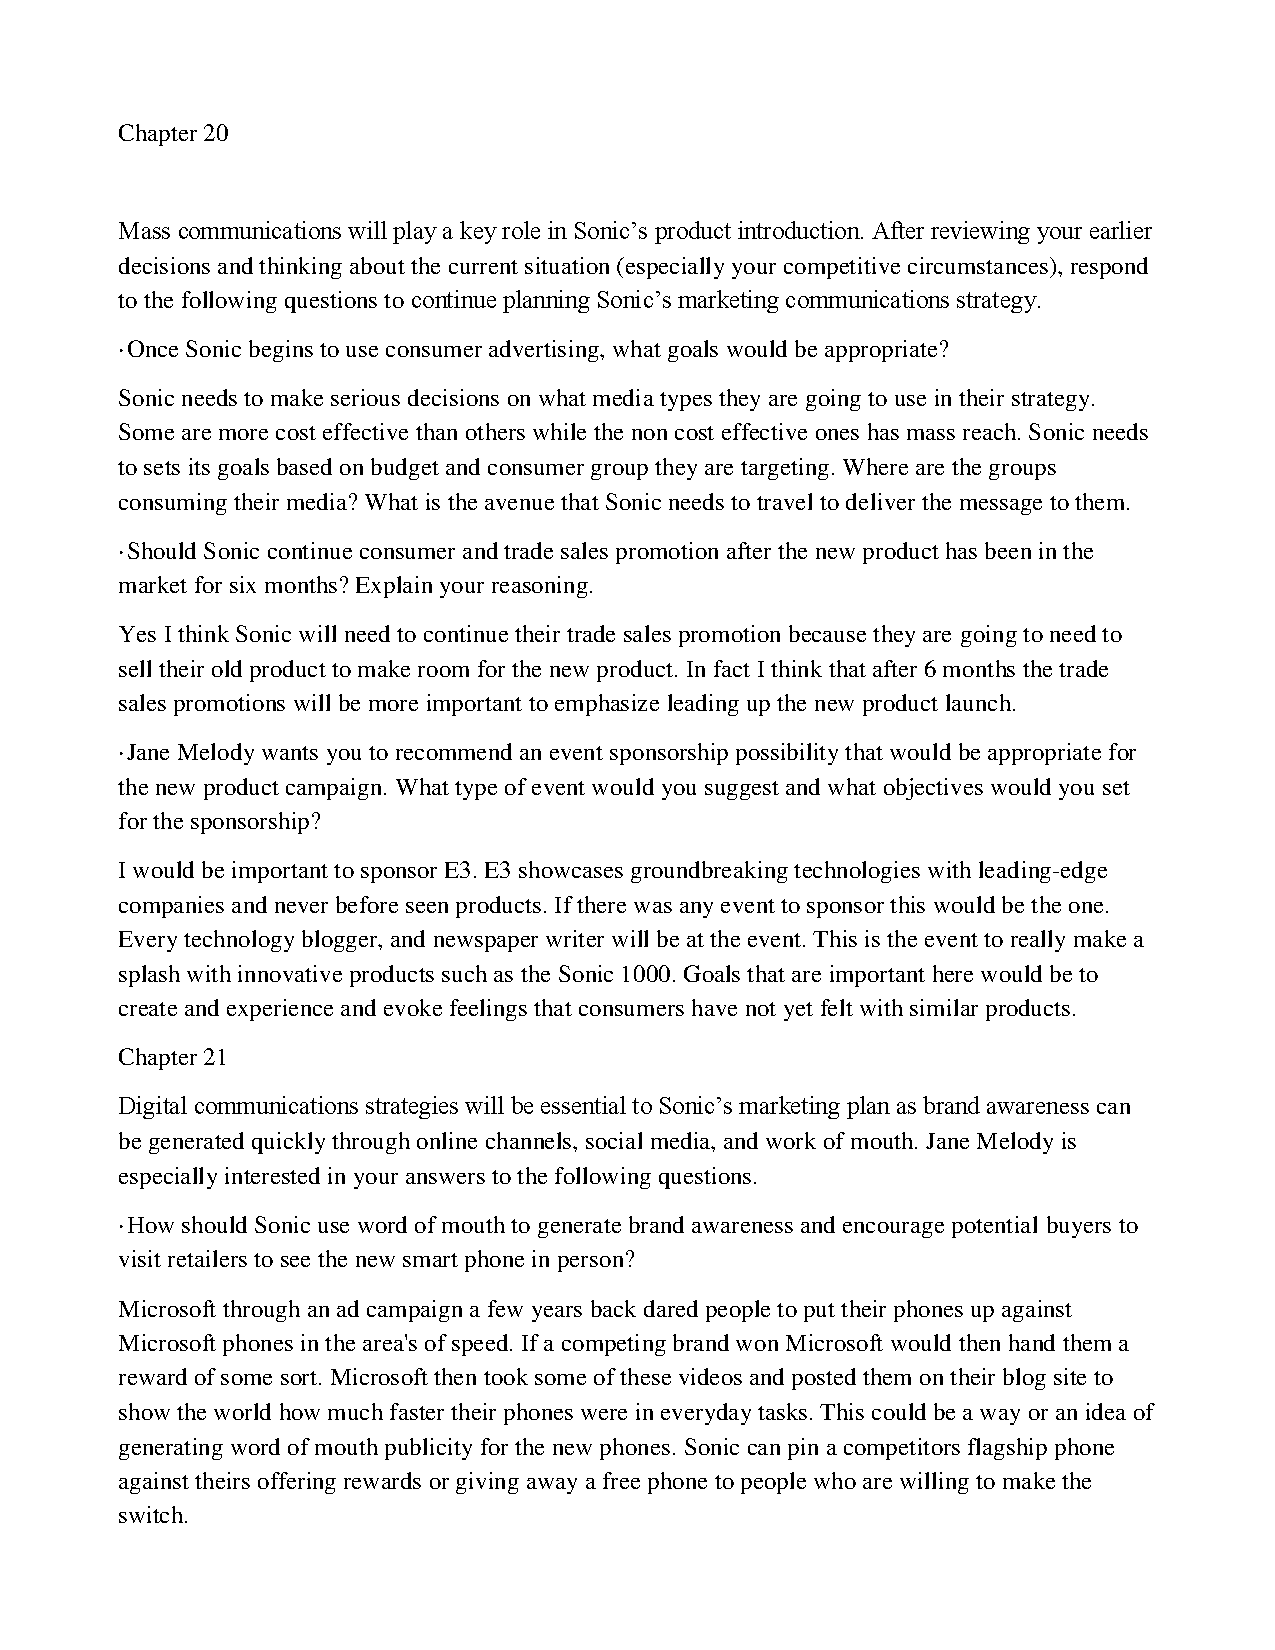
\includepdf[pages=1, pagecommand={\subsubsection{Work Examples}}]{week_7.pdf}
\restoregeometry
\includepdf[pages=2-]{week_7.pdf}
% Spring 2016
\subsection{Business Internship}
\subsubsection{Reflections}
\paragraph {}
The graduate internship was a great experience that allowed me to gain real world knowledge and tie it in with classroom studies. This was the last course I had to take. I wanted to save this for last so I would not have any other studies taking valuable time where I could spend my time comprehending the entire internship process.
\paragraph {}
I chose to do my internship with a small business because I was aligning my after school goals with school experience. I wanted to see first hand what challenges a company of this size has and wanted to learn how a small business can compete against large scale organizations. I feel that during my time with the company I have learned the strengths and weaknesses of small organizations. Most of the differences revolved around money issues. Large organizations tend to have more money to throw at marketing for customer acquisition and can spend more needed software infrastructure. These two topics make the small business owner feel they cannot compete in the same retail space. What I learned is that the small business offers greater flexibility than the large competitors. This presents great opportunities for the business to sway customers by offering what they are needing on an individual basis. Something that cannot happen in a large organization.
\paragraph {}
I really liked how the internship program was structured. It allowed for the student to define how and what they wanted to learn. At time during the entire semester It did not feel like I was at school. I would have enjoyed and sometimes needed the weekly check-ins. I feel that this would be good just to ensure that we are kept on track with our weekly writing. Otherwise this was a great opportunity for me to make a great impression on a great company. I felt that saving this for last was a great cap on the entire masters program and would turn around and perform the internship again.


\includepdf[pages=1, pagecommand={\subsubsection{Work Examples}}]{internship_portfolio.pdf}

\includepdf[pages=2-]{internship_portfolio.pdf}



% Part 3
\section{Part III}
\subsection{Summary and Conclusion}
\paragraph {}
Starting with my enrollment with and acceptance into the graduate program I was really unsure of myself and my abilities to perform at this level. My academic career started with a Associates degree from Western Dakota Technical Institute then finishing my Bachelors degree at National American University. I was worried that National American University wasn't a school that would have prepared me for the journey that I was about to undertake. I feared that maybe the public opinion of the school was correct that it was a diploma mill. Well It's not, my education I received there prepared me for my next academic journey.
\paragraph {}
Since I was unsure of academic my abilities I thought that my first semester was going to break me and thought that I would be seen as not ready this level of classes. I was pleased to find myself in Dr. Blundells class. She did a lot to help me get over the initial jitters of graduate studies. By the end of her class I felt confident that I knew what I was doing and made the right decision to pursue this degree path. I have to admit that my academic writing is still not where it should be to be considered professional but I have come along way since starting this journey.
\paragraph {}
My time with the school has been a joy. The staff and faculty have been great to work with even in times of emergency. This became apparent during a blizzard in October 2013 when I did not have power or the ability to leave my property for over 10 day. Everyone worked with me so I could still turn in assignments even if they were late. Everyone then worked closely with me in February of 2014 when my mother passed away. This was a difficult time and again the faculty work with me so I could turn in assignments late.  These instances showed me that everyone in this school cares about their students and wants to see us succeed in our academic careers. In contrast My wife attends a different school. During the blizzard her teachers were not willing to work with her and gave reasoning that she should have turned her assignments in earlier then. So I want to say thank you. This school shows great compassion for their students.
\paragraph {}
After my mothers passing I found little motivation to want to move forward with school. I started the journey because of her wanting to prove myself semester after semester. I may have wanted to quit but I am glad I have stuck with it to the finish line. I have said this many times that I wanted this degree path because the people in the organization is what make the company. Throughout the courses that I have taken I feel that this philosophy still holds true. The programs core offerings focused around working with the people showing that there is no more important asset to a company the their people. I now feel more eager than ever to share this experience in the workforce developing employees and organizations to hold better knowledge of each other.
\paragraph {}
During my academic career my thoughts and goals may have changed. When I started at Western Dakota Technical Institute my goal was to work as a professional firefighter. Then I slowly started to change. As time moved on it became apparent that what I wanted was to own my own company. I wanted to create the organizational culture that I wanted. During my time with Chadron State College I feel that I have moved ever closer to this goal. This was the basis for my internship. I wanted to be in the capacity of a small business and learn how they cope with business challenges. I learned from this that small business need to handle these challenges in a vary different way than large organizations. What it doesn't mean is that the concepts applied should be different. After completing the internship I am confident that the teachings where preparing us for the major decisions that come from running a business either small or large. The trick is figuring out how to apply the concepts from the last three years.
\paragraph {}
In sum the last three years have been wonderful and I would have never expected to have come this far academically. This school along with their faculty are outstanding causing me to suggest this school to anyone who asks. I am now more prepared and cognoscente of the business world. There may have been classes or parts of classes that I did not like or care for. But there was not a single class that was a waste of time. Each offering had validity when speaking in terms of what is needed in the professional arena. My largest criticism is not of this school but rather on the standards of online learning. There needs to be a better bridge between the classroom and the computer screen. One suggestion is to have in class lectures taped and posted online for students to watch. This might help the visual learners who are taking classes online. This has been a great journey and thank you for my continued and future success.



\end{document}
